% !TEX encoding = UTF-8
% !TEX TS-program = pdflatex
% !TEX root = ../tesi.tex
% !TEX spellcheck = it-IT

%**************************************************************
\chapter{Svolgimento dello stage}
\label{cap:progetto}
%**************************************************************

\intro{In questo capitolo verranno descritti i dettagli riguardanti
l'attività di stage.}\\

%**************************************************************
\section{Pianificazione}\label{sec:prog-pianif}

Man mano che le definivo, di settimana in settimana ho inserito le attività
pianificate in sprint visibili solamente a me in JPA.

In questi sprint ho creato e assegnato a me stesso i task, utilizzando i tipi
disponibili nel seguente modo:

\begin{itemize}
\item \textbf{Nuovo sviluppo:} documentazione
\item \textbf{Implementazione:} realizzazione di funzionalità
\item \textbf{Errore:} anomalie riportate dal tutor aziendale o dagli altri
  membri del team
\end{itemize}

Sebbene dalla quarta settimana fossero disponibili anche le checklist per
pianificare ed organizzare il proprio lavoro, non ho mai avuto necessità di
utilizzarle siccome gli sprint da me utilizzati erano personali. A causa
di ciò, la visualizzazione dello sprint rimaneva chiara anche decomponendo i
task più complessi in un insieme di task.

La pianificazione effettuata durante l'attività di stage ha raffinato gli
obiettivi ed il Piano di Lavoro inizialmente individuati.

Dal momento che durante lo stage ho completato anticipatamente alcune parti
del lavoro previsto, sono stati aggiunti nuovi obiettivi produttivi ad
attività in corso.

Le deviazioni rispetto al Piano di Lavoro (tabella \ref{tab:piano-di-lavoro})
delle otto settimane lavorative di stage sono riportate in tabella
\ref{tab:deviazioni}.

Si può in particolare notare che la maggior parte del lavoro svolto nelle
settimane 5, 7 e 8 non era prevista inizialmente. Ho concordato questi
incrementi con il tutor aziendale durante la mia permanenza a Sanmarco
Informatica, analizzando ulteriori necessità del team.

\begin{tabular}[t]{| c | p{10cm} |}

\hline
\textbf{Settimana} & \textbf{Lavoro effettuato} \\
\hline
1 &
Sviluppo di un layout alternativo per un modulo (non previsto). \\
\hline
2 &
Mancato sviluppo di creazione checklist da template (obbligatorio) e
  importazione template in checklist (opzionale). \\
\hline
3 &
Sviluppo creazione checklist da template (in ritardo dalla settimana 2). \\
\hline
4 &
Completamento modulo burn-down chart, documentazione esclusa. \\
\hline
5 &
Importazione di template in checklist (opzionale, in ritardo dalla settimana
  2). Completamento documentazione burn-down chart. Sviluppo avvio istanza da
  task Scrum (in anticipo, previsto per settimana 6). Sviluppo di ulteriori
  strumenti di Inspection: burn-up chart, pie chart, cumulative flow diagram e
  una variante del burn-down chart (inizialmente non previsti). \\
\hline
6 &
Analisi, sviluppo e documentazione sul collegamento tra modulo scrum e modulo
  di notifica (anticipato dalla settimana 7). \\
\hline
7 &
Analisi, sviluppo e documentazione sul collegamento tra modulo scrum e
  modulo forum (anticipato dalla settimana 8). Sviluppo di \gloss{api} per
  JPAUtil (inizialmente non previste). Implementazione di un nuovo tipo di
  notifica utilizzando un Telegram Bot. \\
\hline
8 &
Sviluppo di un sistema di gestione del collegamento tra il proprio utente e il
  proprio numero telefonico/account su Telegram. Sviluppo di un modulo di
  istruzioni per la creazione di un proprio Telegram Bot. Prototipazione di
  invio di documenti. Incremento in termini di sicurezza dell'accoppiamento tra
  un utente e il Telegram Bot. Studio della realtà aziendale e inizio stesura
  della relazione finale. \\
\hline
\end{tabular}
\captionof{table}{Deviazioni rispetto al Piano di Lavoro}
\label{tab:deviazioni}

\paragraph{Strumenti di \emph{Inspection}} \mbox{} \\

Un burn-down chart può non essere l'unico strumento di \emph{Inspection} utile
per un gruppo di lavoro, poichè non riesce a mostrare informazioni riguardo a
diversi indicatori di performance:

\begin{itemize}
\item un \textbf{burn-up chart} mostra quante attività vengono aggiunte man
  mano che lo sprint avanza, mettendo in evidenza eventuali lacune
  nell'attività di pianificazione;
\item un \textbf{cumulative flow diagram} mostra i livelli in cui risiedono
  maggiormente i task, trovando eventuali colli di bottiglia nei processi di
  sviluppo aziendale e permettendo di ricavare utili informazioni come il
  \gloss{lead-time}.
\end{itemize}

\paragraph{Notifiche su Telegram} \mbox{} \\

Le funzionalità di notifica previste dal Piano di Lavoro riguardavano l'invio
di mail interne tramite un modulo di JPA dedicato a tale scopo.

Tuttavia, tale parte dell'applicazione è ancora in via di sviluppo e presenta
delle limitazioni come il fatto di non poter essere utilizzata al di fuori di
JPA.

Per questo motivo, durante lo stage ho concordato con il tutor aziendale lo
sviluppo di un nuovo tipo di notifiche, trasmesse su Telegram.

Telegram è un programma di messaggistica istantanea completamente
gratuito\footnote{A differenza di altri software, anche le \gloss{api}
disponibili sono gratuite} che ha nella velocità e nella sicurezza i suoi
punti di forza. Questa applicazione è disponibile sia su dispositivi mobili
che su computer ed è permesso l'invio di qualsiasi tipo di file.

Dal 24 giugno di quest'anno Telegram ha reso disponibile i \textbf{Telegram
Bot}, ovvero degli account che ricevono e inviano messaggi via software e non
per comando diretto di persone.

Grazie a questi Bot è quindi possibile automatizzare attività e, nel caso del
mio stage, inviare messaggi contenenti notifiche relative ad eventi su JPA.

%**************************************************************
\section{Norme e strumenti}

\subsection{Formazione delle conoscenze mancanti}

Per formare le conoscenze mancanti ho proceduto sia con un apprendimento di
tipo teorico, consultando video on-line, libri e articoli di blog, sia con un
apprendimento di tipo pratico.

Questo mi ha permesso di conoscere Scrum, come i metodi agili sono collegati
al resto dei metodi di produzione industriale e di apprendere le
\gloss{best-practice} per le tecnologie che non conoscevo.

\subsection{Comunicazione tra membri del team}

Le interazioni tra membri del team avvengono tramite diversi mezzi di
comunicazione:

\begin{itemize}
\item dialogo verbale, per analisi o chiarimenti veloci e di importanza minima.
  Gli esiti di questa venivano riportati per iscritto;
\item Telegram, per comunicazioni veloci di carattere generico;
\item Skype, per condivisione di file leggeri e link;
\item forum di JPA, per la discussione di tematiche di sviluppo di interesse
  comune all'intero team;
\item note su task in JPA, per aggiungere brevi notizie relative ad uno
  specifico task;
\item mail interna a JPA, utilizzata solamente per le prime settimane di stage
  per comunicare l'ultimo numero del messaggio di errore per il lato client di
  JPA;
\item mail personale (esterna a JPA), per comunicazioni di carattere formale.
\end{itemize}

\subsection{Sviluppo}

Le norme, le procedure e gli strumenti rispettati per lo sviluppo sono un
sovrainsieme di quanto elencato in sezione \ref{sec:azienda-tecnologie}.

In questa sezione verranno riportati i metodi e le regole che ho imposto a me
stesso durante lo sviluppo, facendo particolare attenzione che questi non
fossero conflittuali con quanto imposto dall'azienda.

\paragraph{Analisi} \mbox{} \\

L'attività di \textbf{analisi} serviva a delineare i requisiti e i possibili
scenari di applicazione per una funzionalità da introdurre.

Per quanto riguarda i requisiti, ho diviso questi in:

\begin{itemize}
\item \textbf{Requisiti funzionali:} condizioni il cui soddisfacimento
  comportano un adempimento di una caratteristica comportamentale del sistema
  (e.g. aggiunta della funzionalità di modifica elemento). Tali requisiti hanno codice RFX(.Y(.Z))Imp
\item \textbf{Requisiti non funzionali:} condizioni il cui soddisfacimento
  comporta un miglioramento della qualità d'uso del prodotto sviluppato (e.g.
  realizzazione del Manuale Utente). Tali requisiti hanno codice
  RNFX(.Y(.Z))Imp
\end{itemize}

A loro volta, i codici per i requisiti hanno i seguenti parametri:

\begin{itemize}
\item X, Y e Z sono dei numeri progressivi che partono da 1 per ogni sviluppo
  effettuato;
\item \textbf{Imp} è un codice che discrimina l'importanza di un requisito:
  ``Obb'' sta per obbligatorio, ``Opz'' sta per opzionale ed infine ``Des''
  corrisponde a desiderabile.
\end{itemize}

I requisiti individuati venivano a loro volta frammentati fino a diventare di
granularità tale da poter monitorare con precisione il loro soddisfacimento,
per entrambi i tipi di requisito.

Per quanto riguarda i casi d'uso, li ho realizzati per poter dialogare con
minor ambiguità con il tutor aziendale riguardo gli obiettivi da
definire.

Ho delineato i casi d'uso solamente per gli obiettivi più complessi,
esplicitando solamente le funzionalità più critiche di questi. Lo standard
adottato per la stesura di questi è \gloss{uml} 2.0.

\paragraph{Progettazione} \mbox{} \\

A seguito dell'analisi vi è l'attività di \textbf{progettazione}.

JPA presenta un'architettura progettata per essere facilmente estensibile in
caso di modifiche di lieve entità: nella maggior parte dei casi,
l'implementazione di nuove funzionalità richiede la riproduzione di componenti
architetturali già esistenti, sia nel lato client che in quello server.

Per questo motivo, la progettazione ha (almeno inizialmente) seguito il flusso
rappresentato in figura \ref{fig:progettazione}.

L'unico caso particolare presente in questa procedura è, come si può vedere,
quando dovevo introdurre una nuova componente nel \FREND{}: ciò avveniva quando
l'implementazione delle modifiche richiedeva l'aggiunta di una nuova area, un
modulo o un componente riusabile in più moduli come una \gloss{direttiva}.

Per realizzare la struttura di tali componenti, mi è stato sufficiente
ispirarmi a quelle simili già esistenti: in questo modo, gli incrementi
che ho introdotto durante lo stage sono facilmente manutenibili dal resto del
team.

\begin{figure}%
\centering
\includegraphics[width=.8\columnwidth]{immagini/progettazione}
\caption{Procedura utilizzata durante la progettazione}
\label{fig:progettazione}%
\end{figure}

Eventuali diagrammi delle classi sono stati realizzati seguendo lo standard
\gloss{uml} 2.0.

Tuttavia, vi sono state delle eccezioni a questa procedura di progettazione.

La prima consiste nello sviluppo delle funzionalità di notifica: l'architettura
da progettare per questa parte doveva presentare un livello di complessità
maggiore affinchè potesse essere estesa più facilmente in futuro.

Oltre a ciò, col passare delle settimane la mia conoscenza su AngularJS è
cresciuta con studi personali. Finchè lavoravo sulla parte di \FREND{} nelle
prime cinque settimane, ho notato che il principio DRY\footnote{\emph{Don't
Repeat Yourself}} non veniva rispettato: molte parti di logica applicativa del
lato client venivano replicate in diversi moduli, sebbene fossero relative non
a uno specifico modulo, ma ad una componente specifica del dominio applicativo.

Per questo motivo, ho introdotto nell'architettura del \FREND{} degli
\emph{Angular service}, ovvero oggetti che potessero incapsulare delle
operazioni specifiche per un certo elemento del dominio applicativo (e.g.
collegamento tra area forum e uno sprint).

Con questo approccio, fin da subito ho avuto vantaggi significativi:

\begin{itemize}
\item \textbf{Diminuzione delle righe di codice:} molte parti di codice lunghe
  e ripetute sono state spostate esternamente ai moduli, alleggerendo questi;
\item \textbf{Costo delle modifiche:} anzichè dover cercare le sezioni di
  codice in cui le stesse istruzioni venivano eseguite, è stato sufficiente
  applicare una modifica al corpo dei \emph{service};
\item \textbf{Aderenza al \gloss{framework}:} L'architettura di AngularJS è
  spesso definita come MVVM (\emph{Model-View-ViewModel}). Il controller e
  l'oggetto \texttt{\$scope} (i quali insieme compongono il ViewModel)
  dovrebbero fornire solamente uno strato intermedio tra vista e modello.
  Nell'architettura del \FREND{} pre-esistente, il controller stesso aveva al
  suo interno l'intera \emph{business logic} e la parte di Model era
  completamente assente.
\end{itemize}

\begin{figure}[H]%
\centering
\includegraphics[width=.7\columnwidth]{immagini/mvvm}
\caption{Schema architetturale di Model-View-ViewModel}
\source{\url{https://i-msdn.sec.s-msft.com/dynimg/IC564167.png}}
\label{fig:mvvm}%
\end{figure}

\paragraph{Codifica} \mbox{} \\

Una volta conclusa la progettazione, comincia l'attività di codifica. Per
questa attività ho individuato regole aggiuntive rispetto a quelle già
impiegate dal team.

Per il \BKEND{} ho deciso di commentare con Javadoc ogni classe, campo dati o
metodo qualora il nome di questi non facesse già capire cosa rappresenta tale
entità.

Tale accorgimento è stato veramente utile, poichè molte classi presentavano
molti campi dati con nomi lunghi due o tre lettere (per motivi di efficienza)
e l'\gloss{ide} in assenza di Javadoc non fornisce un aiuto contestuale per la
loro descrizione.

Se ad essere commentata è un'operazione, ho deciso di utilizzare anche le
annotazioni \texttt{@param} e \texttt{@return} (e talvolta \texttt{@throws})
per spiegare quali parametri fornire e cosa restituisce tale metodo.

Un altro accorgimento adottato per il \BKEND{} è far corrispondere ad ogni
variante di una classe enumerativa una stringa che la rappresenti.

Per il \FREND{} ho adottato le seguenti convenzioni:

\begin{itemize}
\item per la dichiarazione di oggetti vuoti, inizializzarli dando come valore
  \texttt{\{\}};
\item per la dichiarazione di vettori vuoti, inizializzarli dando come valore
  \texttt{[]};
\item uso di JSDoc per i metodi più complessi;
\item il nome di ciascuna collezione in cui si raggruppano diversi servizi
  deve terminare con \texttt{Services}.
\end{itemize}

Oltre alle regole sopra elencate, per il \FREND{} ho deciso di versionare
autonomamente quanto producevo. Il \gloss{vcs} che ho scelto è \textbf{Git},
siccome avevo già esperienza con tale sistema.

Questo mi ha permesso di:

\begin{itemize}
\item avere un ramo principale (\texttt{master}) in cui sono presenti tutti
  gli incrementi per i vari obiettivi previsti dal Piano di Lavoro;
\item avere dei rami secondari per funzionalità il cui inserimento non
  garantiva stabilità (ad esempio quando ho inserito gli
  \emph{Angular service} ho creato un ramo apposito);
\item alla consegna del lavoro, ho potuto inviare al tutor aziendale una copia
  del \gloss{repository} in cui vi è una sequenza di salvataggi
  sufficientemente o più granulare da poter separare la realizzazione di un
  obiettivo da un altro. In questo modo, l'inclusione dei vari
  incrementi è molto più semplice sia in termini di integrazione che di
  verifica;
\item avere una \emph{staging area}, in cui salvare temporaneamente e non
  definitivamente le modifiche, per poterle confermare in un secondo momento
  (al contrario di SVN, dove questa è assente).
\end{itemize}

\paragraph{Documentazione} \mbox{} \\

Per la documentazione ho utilizzato il linguaggio \LaTeX{}, \TeX{}Studio come
ambiente di scrittura, Modelio per i diagrammi UML e Inkscape per trattare le
immagini da inserire.

I documenti possono essere:

\begin{itemize}
\item Manuali Utente;
\item Specifiche Tecniche;
\item documenti di carattere generico.
\end{itemize}

Per ogni documento, ogni revisione deve essere indicata e, nel caso in cui vi
sia più di una revisione dello stesso documento, deve essere inserito un
diario delle modifiche.

Ciascun documento ha una sezione introduttiva, dove è indicato lo scopo del
documento, lo scopo del prodotto, istruzioni per la lettura del documento (ad
esempio vengono esplicitate eventuali convenzioni tipografiche o l'uso di
standard come \gloss{uml}) ed eventuali note sulla parte di prodotto descritta.

Ciascun documento possiede un glossario, collocato nelle pagine finali e
avente contenuto specifico per il dominio applicativo trattato.

%**************************************************************
%**************************************************************
%**************************************************************
%**************************************************************
%**************************************************************
\section{Resoconto dell'attività di stage}

\subsection{Formazione}

Lo stage è cominciato investendo del tempo per apprendere le conoscenze
mancanti per poter svolgere al meglio il lavoro.

Ho speso il tempo della prima settimana nel seguente modo:

\begin{itemize}
\item 50\%: lettura libri, articoli di blog e video su Scrum, AngularJS e
  Bootstrap;
\item 35\%: sviluppo template di documento in \LaTeX{} e del primo documento
  (riguardante lo studio della metodologia Scrum e le differenze tra la teoria
  e quanto offerto attualmente dall'area Scrum di JPA);
\item 10\%: sviluppo di un layout alternativo per una View HTML per prendere
  confidenza con i \gloss{framework} del \FREND;
\item 5\%: spiegazione del \emph{workspace} da parte del tutor aziendale;
\end{itemize}

Questa preparazione iniziale è stata fondamentale per il resto dello stage: ho
infatti evitato di cominciare ad utilizzare le tecnologie senza conoscerle
sufficientemente e il costo di produzione dei documenti è stato notevolmente
ammortizzato nelle settimane seguenti.

\subsection{Analisi}

Al fine di definire al meglio gli obiettivi produttivi, all'inizio di ciascuno
sprint ho effettuato con il tutor aziendale un'attività di analisi, mirata a
capire i bisogni degli \emph{stakeholders} (il resto del team).

\paragraph{Checklist} \mbox{} \\

Il primo obiettivo era legato allo sviluppo di checklist, ovvero liste che
possono essere popolate con una serie di voci in modo tale da poter elencare
delle micro-attività, la cui esecuzione comporta il completamento
dell'attività che queste compongono in una visione d'insieme.

In particolare, erano previsti un modulo per gestirle e una \gloss{direttiva}
per includerle all'interno di altri moduli.

Il modulo relativo alle checklist doveva offrire le seguenti funzionalità:

\begin{enumerate}
\item creare un template di checklist;
\item creare una checklist;
\item importare un template in una checklist.
\end{enumerate}

La \gloss{direttiva} doveva fornire una componente da includere in altri
moduli. Durante lo stage, ho incluso questa componente nel visualizzatore di
sprint, in modo tale che fosse disponibile per ogni task.

In questo modo, era possibile selezionare una checklist da collegare ad un
task e utilizzarne le funzionalità direttamente da tale vista.

La tabella dei requisiti per le funzionalità relative a checklist non viene
riportata, poichè ridonderebbe informazioni banali o già enunciate qui sopra.
Tuttavia, ho deciso di riportati i requisiti funzionali che non appaiono
evidenti da quanto finora esposto:

\begin{enumerate}
\item le righe di template di checklist possono essere obbligatorie o
  opzionali;
\item le righe di template di checklist possono essere modificabili o
  importabili in sola lettura;
\item il modulo di gestione checklist deve visualizzare diverse liste di
  checklist a seconda del filtro applicato: le possibili scelte sono
  ``Nuove'', ``Mie'', ``Attive'' e ``Completate'';
\item dev'essere possibile cambiare la posizione di righe di checklist;
\item le checklist e i template di checklist non possono mai essere eliminati
  fisicamente ma al più disattivati.
\end{enumerate}

\paragraph{Burn-down chart} \mbox{} \\

I burn-down chart sono dei grafici utilizzati per studiare l'andamento del
lavoro in un team.

Il lavoro residuo è espresso in percentuale: ad inizio sprint parte dal
valore 100\%, mentre ci si aspetta che nel giorno di fine sprint la
percentuale abbia raggiunto lo 0\%.

I grafici sono così composti (si veda figura \ref{fig:bdchart}):

\begin{enumerate}
\item sull'asse delle ascisse sono riportati i giorni che vanno dall'inizio
  dello sprint fino alla sua fine;
\item sull'asse delle ordinate è presente la percentuale di lavoro rimanente;
\item sulla legenda sono indicati i dati visualizzati nel diagramma, con i
  relativi colori con cui sono stati disegnati;
\item la retta ideale parte da 100 (il primo giorno) e arriva ad esaurirsi
  completamente a fine sprint;
\item la curva reale viene calcolata interpolando le unità di lavoro
  disponibili per tutti i giorni non posteriori alla data corrente;
\item le colonne sono composte sovrapponendo i vari carichi di lavoro
  residuo\footnote{Il valore residuo per ogni task dipende dal livello di
  avanzamento in cui esso si trova} per ogni tipo di task.
  \begin{itemize}
  \item nella visualizzazione per tipi, ogni colonna e relativo tooltip sono
    colorati con la tonalità associata ad un certo tipo;
  \item nella visualizzazione per livelli, ogni tooltip ha al suo interno ha
    l'icona associata al livello corrispondente.
  \end{itemize}
\end{enumerate}

Durante l'attività di stage ho dovuto sviluppare una \gloss{direttiva} che
fosse integrabile in altri moduli, in modo tale che questa mostrasse un
burn-down chart una volta ricevuto il codice identificativo dello sprint da
analizzare.

\begin{figure}[H]
  \subfloat[Visualizzazione per tipi\label{fig:vis-tipi}]{%
    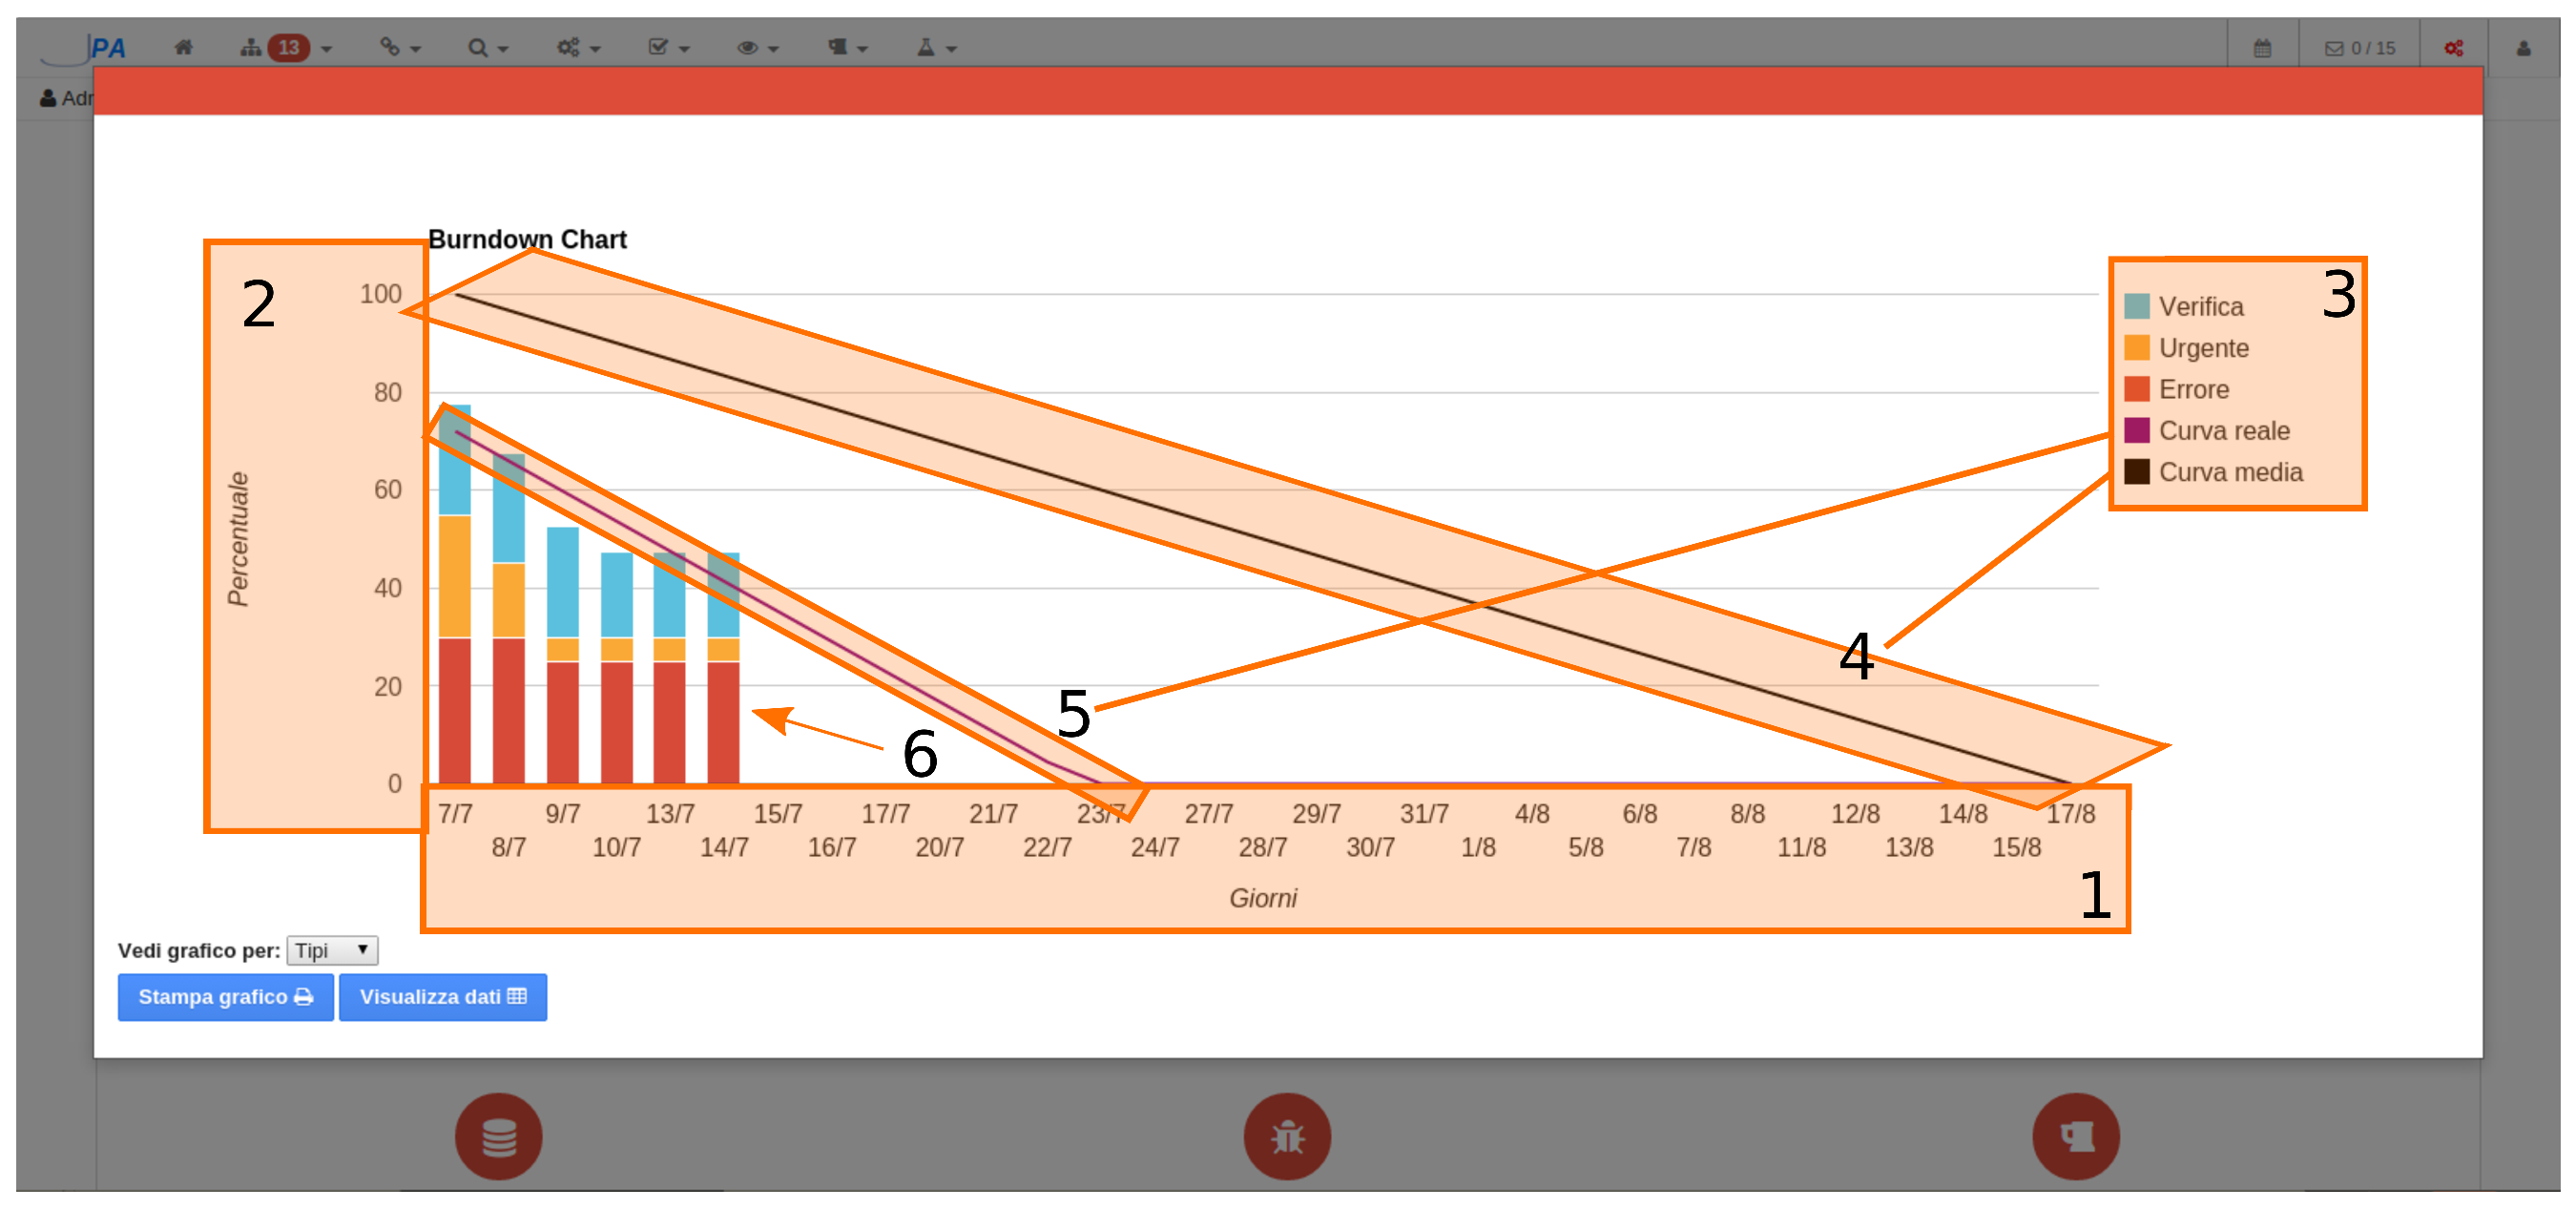
\includegraphics[width=\textwidth]{immagini/EAAPartiDelChart}
  }
  \vspace*{\fill}
  \subfloat[Visualizzazione per livelli\label{fig:vis-levs}]{%
    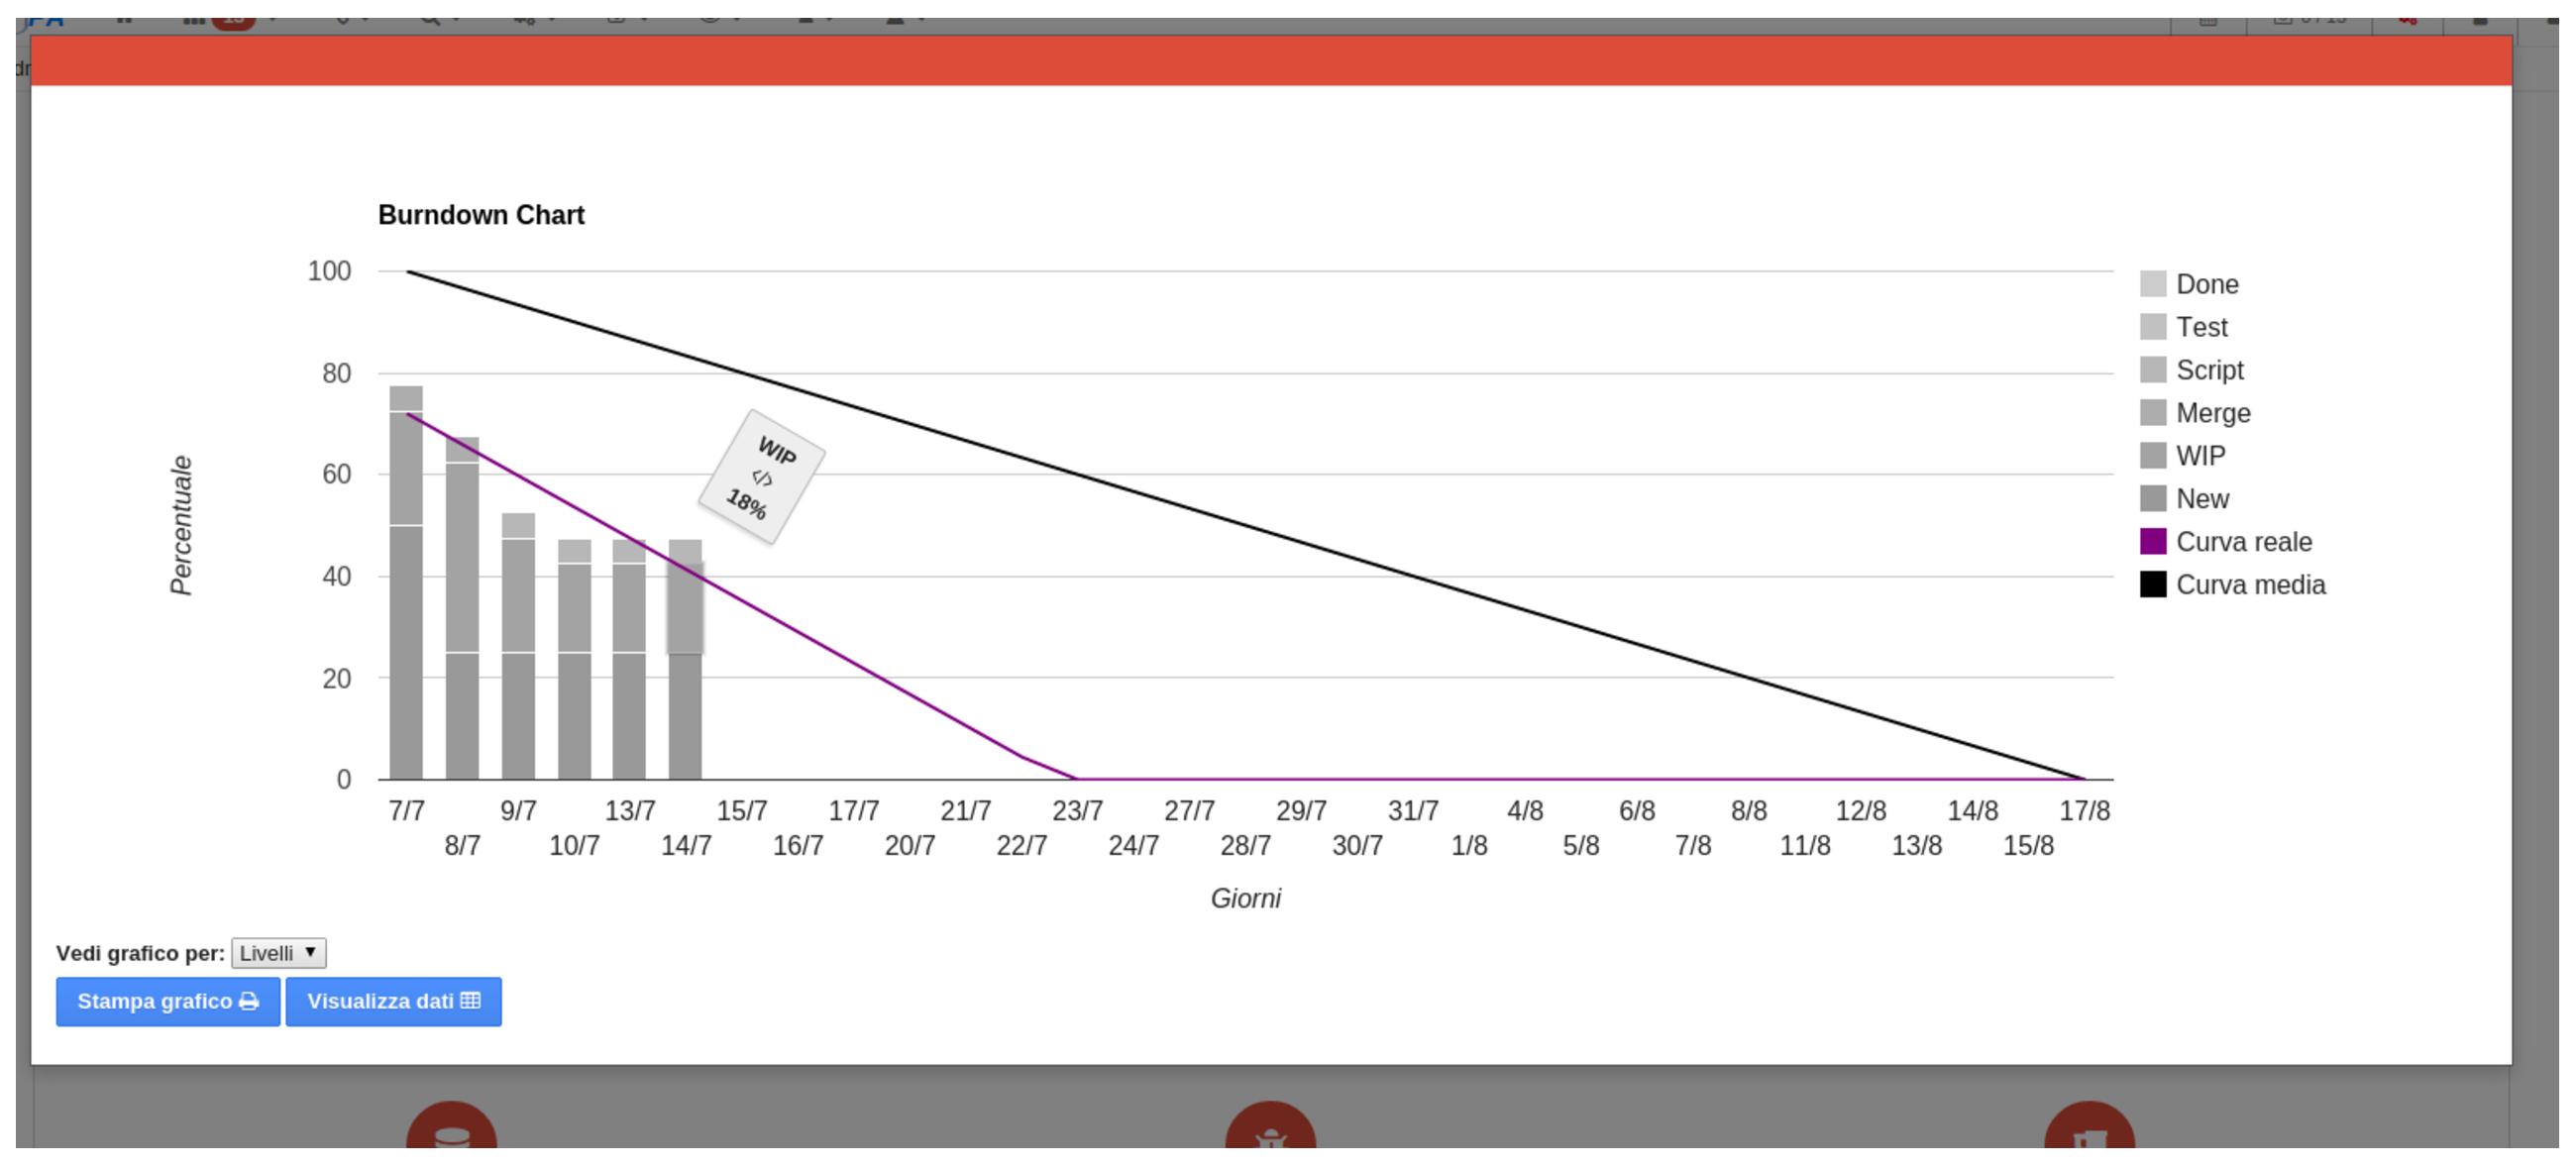
\includegraphics[width=\textwidth]{immagini/FACVediTooltipLivelli}
  }
  \caption{Burn-down chart}
  \label{fig:bdchart}
\end{figure}

La tabella dei requisiti per i burn-down chart non viene riportata, poichè
ridonderebbe informazioni già enunciate in precedenza. Tuttavia, ho deciso di
riportati i requisiti funzionali che non appaiono evidenti da quanto finora
esposto:

\begin{enumerate}
\item il grafico viene tracciato considerando soltanto i giorni feriali della
  settimana (da lunedì a venerdì);
\item i tooltip nella visualizzazione per livelli devono essere colorati con
  tonalità di grigio che sono più chiare più il livello è avanzato;
\item ogni livello corrisponde ad una percentuale di completamento,
  configurabile in un modulo dell'area Scrum;
\item JPA deve offrire la possibilità di stampare il grafico;
\item JPA deve offrire la possibilità di visualizzare i dati del grafico in
  forma tabulare;
\item il carico residuo dei task deve essere proporzionale al numero di spunte
  nella checklist legata al task, se questo:
  \begin{itemize}
  \item si trova in un livello proporzionale a checklist;
  \item è collegato a una checklist.
  \end{itemize}
\end{enumerate}

\paragraph{Strumenti di \emph{Inspection}} \mbox{} \\

Come detto in sezione \ref{sec:prog-pianif}, ho realizzato anche ulteriori
strumenti di \emph{Inspection} per i processi gestiti nell'area Scrum:

\begin{itemize}
\item una variante del burn-down chart, con aree al posto delle colonne;
\item un burn-up chart (fig. \ref{fig:burnup}), che tiene conto dell'aggiunta
  di attività a sprint in corso;

  \begin{figure}[H]%
  \centering
  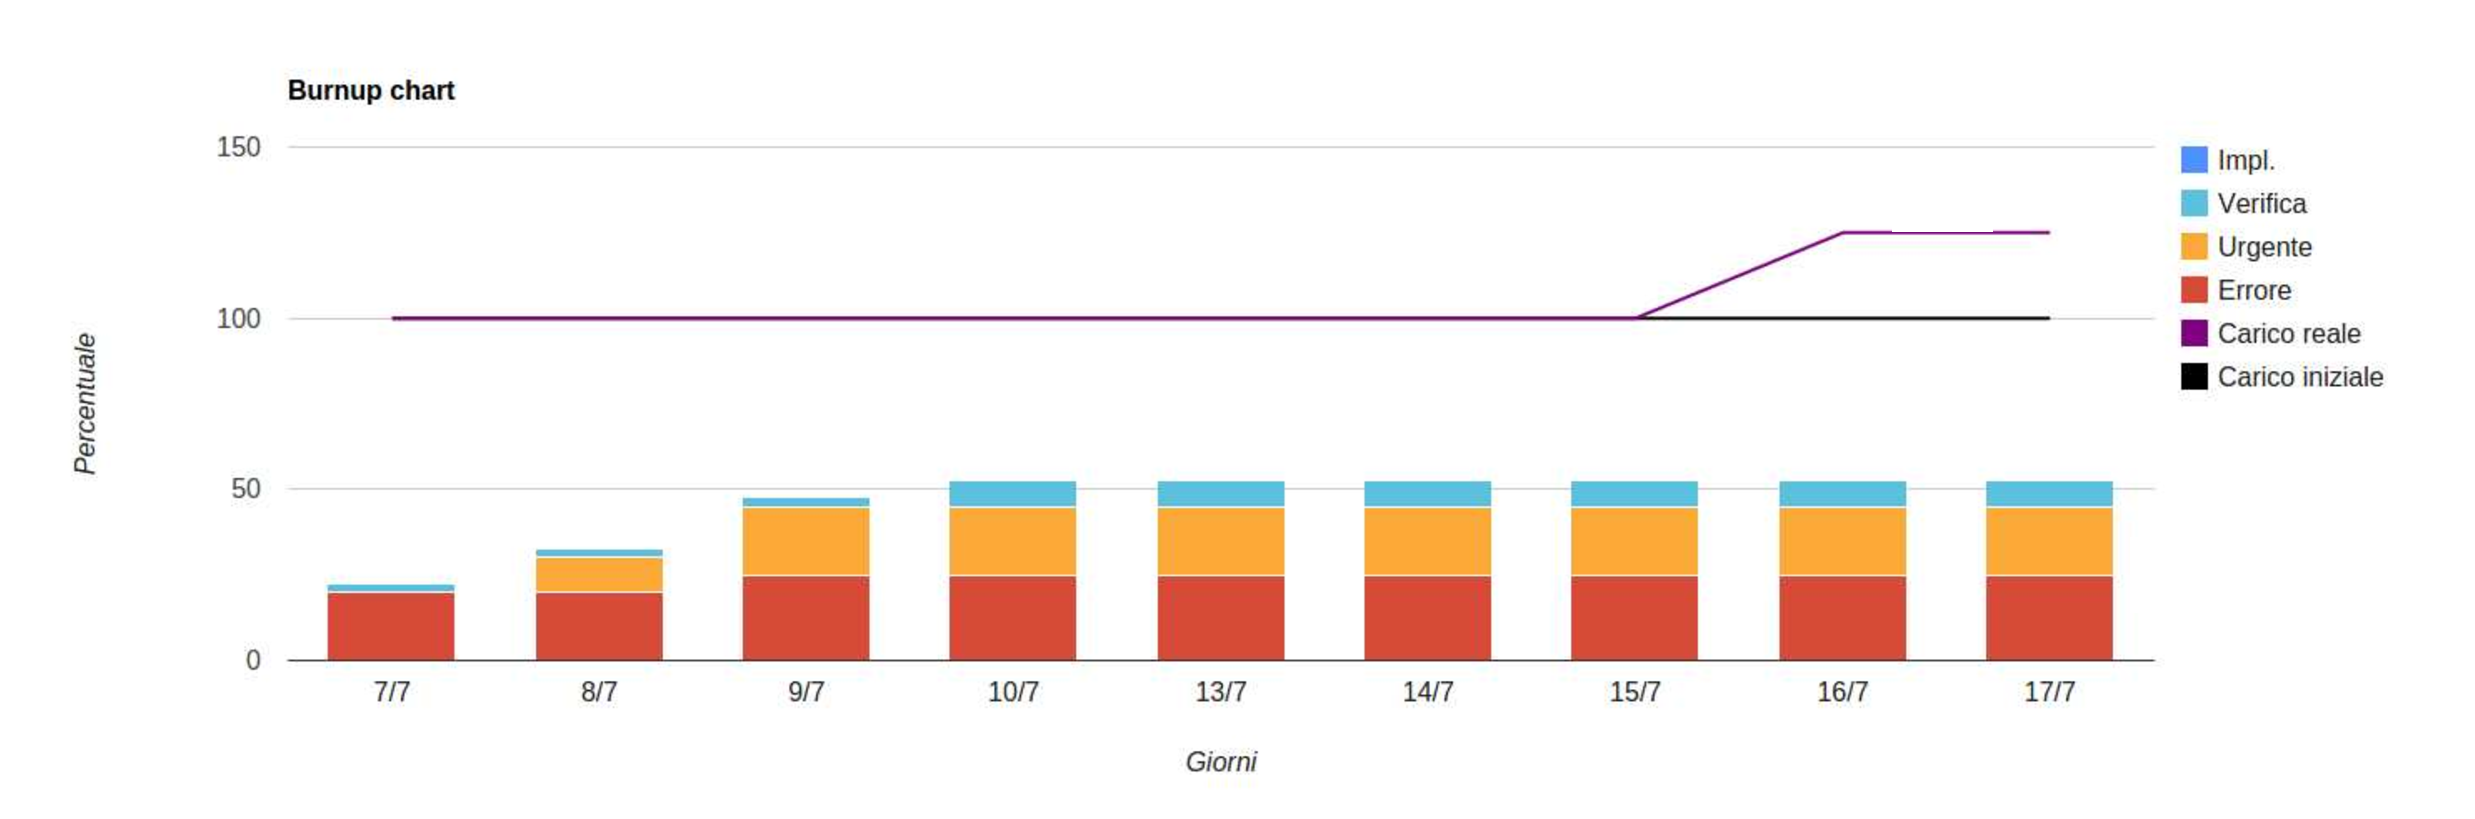
\includegraphics[width=1.1\columnwidth]{immagini/burnup}
  \caption{Burn-up chart}
  \label{fig:burnup}%
  \end{figure}

\item un cumulative flow diagram (\ref{fig:cumulative}), che mostra al termine
  di ciascun giorno quanti task sono in un certo livello;

  \begin{figure}[H]%
  \centering
  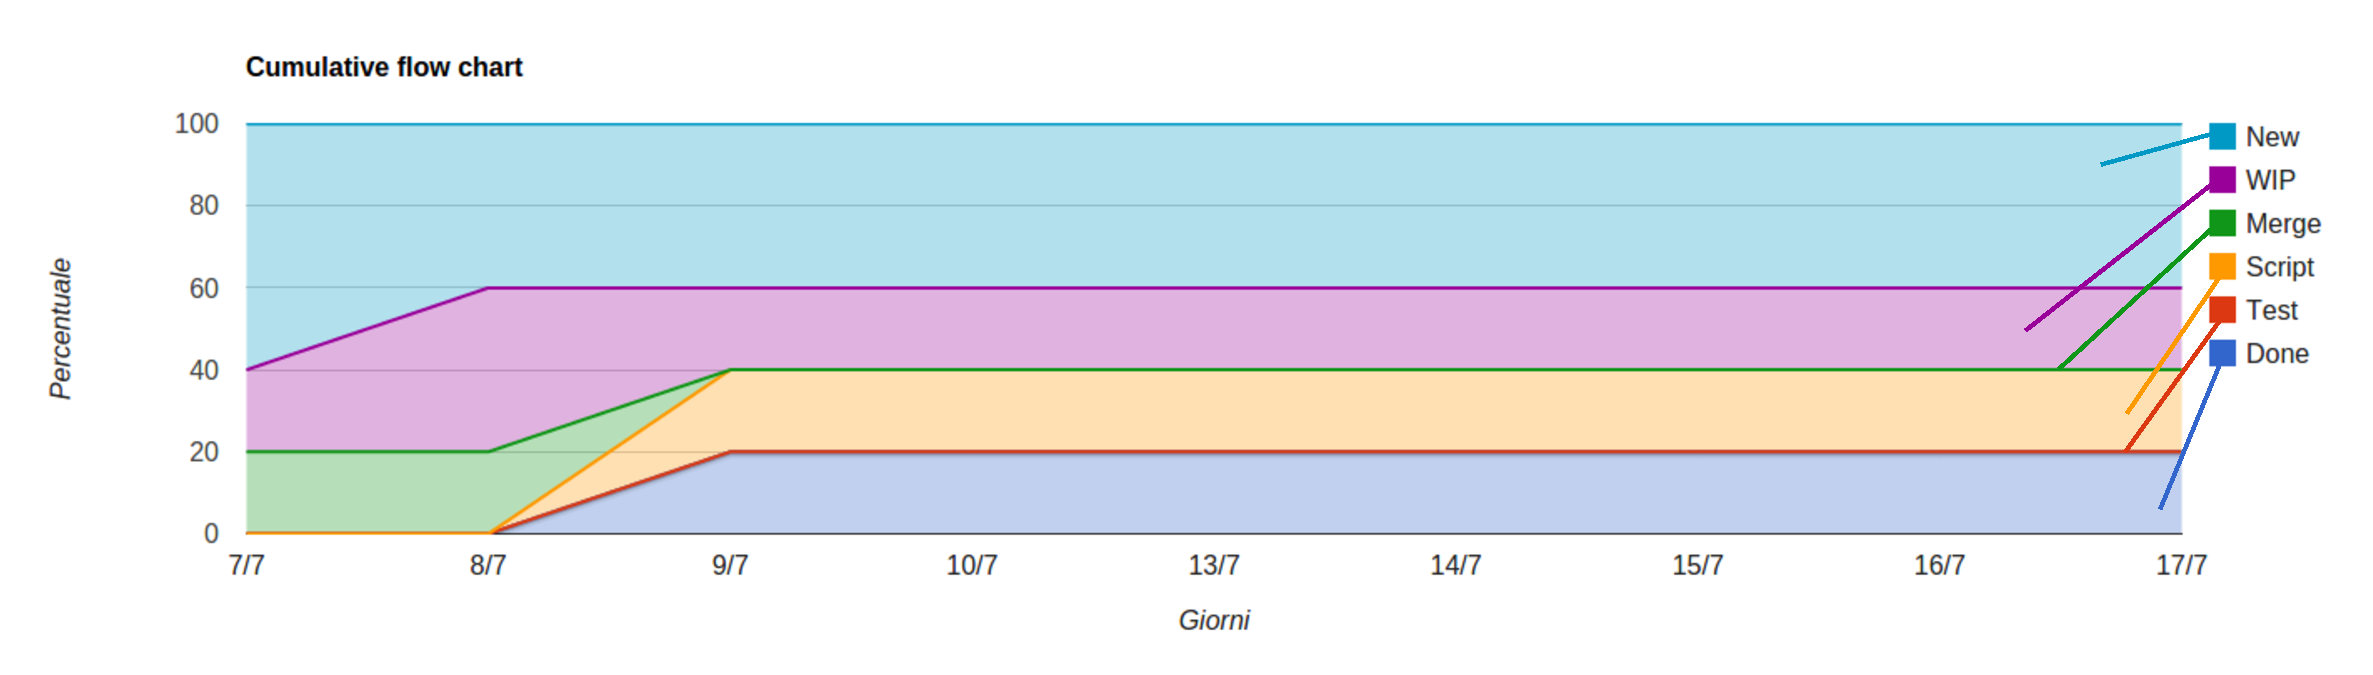
\includegraphics[width=1.1\columnwidth]{immagini/cumulativeFlow}
  \caption{Cumulative flow diagram}
  \label{fig:cumulative}%
  \end{figure}

\item dei pie chart (grafici a torta), per vedere in totale quanti task
  di un certo tipo sono presenti in uno sprint e quanti task sono in ciascun
  livello alla data odierna.
\end{itemize}

Ho inserito questi strumenti in un nuovo modulo, chiamato \gloss{kpi}
dal momento che tramite il loro utilizzo è possibile ricavare misurazioni
riguardo a diversi indicatori (carico di lavoro, costo, tempo di risposta,
etc.).

\paragraph{Avvio istanza di processo} \mbox{} \\

Il primo dei massimi obiettivi produttivi riguardava l'avvio di un'istanza di
processo.

I processi sono un insieme di attività (chiamate task, ma differenti dai task
Scrum), tra cui ci sono sempre le attività \textbf{Start} e \textbf{End}, che
identificano l'inizio e le possibili terminazioni di questo.

Un'istanza di un processo corrisponde ad un'esecuzione di questo e
contemporaneamente è possibile che siano attive più istanze di uno stesso
processo.

Prima dello stage, Scrum e l'area di modellazione e gestione processi erano
totalmente scollegate. Questo poteva rappresentare una limitazione all'uso
del programma, poichè sia utilizzando Scrum completamente che non, potrebbe
essere utile avviare da uno specifico sprint un processo, come una RDA
(richiesta d'acquisto).

Nella descrizione precedente non vengono esplicitati i seguenti requisiti:

\begin{itemize}
\item deve essere possibile visualizzare una lista di processi avviabili per
  gli sprint;
\item deve essere possibile visualizzare una lista di processi avviabili per
  i task Scrum (non per forza uguale alla lista per gli sprint);
\item le liste in cui sono presenti i processi devono essere divise per
  argomento.
\end{itemize}

\paragraph{Realizzazione di \gloss{api} per l'area Scrum} \mbox{} \\

Una volta analizzato l'avvio istanza di processo a partire da un elemento
Scrum, era necessario fornire il collegamento anche nell'altra direzione.

Lo svolgimento di attività dei processi in JPA può avvenire sia manualmente
(da parte di un'operatore) che automaticamente. In questo ultimo caso, risulta
utile fornire delle \gloss{api} per le funzionalità principali dell'area Scrum,
in modo che attività automatiche di processi possano compiere le seguenti
azioni:

\begin{itemize}
\item creazione di sprint (attivo o inizialmente sospeso);
\item sospensione di uno sprint;
\item conclusione di uno sprint;
\item creazione di un task;
\item cambio di livello di un task;
\item inserimento di un task in uno sprint;
\item creazione di log nell'area Scrum.
\end{itemize}

\paragraph{Funzionalità di notifica} \mbox{} \\

Un ulteriore miglioramento previsto era lo sviluppo di funzionalità di
notifica. Queste servono per informare gli utenti di JPA su eventi che
avvengono all'interno dell'area Scrum.

Vi possono essere diverse varietà di notifica, in base al \textbf{tipo} di
queste (ovvero il mezzo con cui vengono trasmesse) e in base
all'\textbf{evento} che causa il loro invio.

Per ciascuna di queste varietà deve essere possibile impostare un titolo ed un
corpo, tenendo conto che all'interno del corpo possono essere presenti delle
\textbf{keyword} (parole chiave). Queste possono essere di tre tipi:

\begin{enumerate}
\item \textbf{Semplici:} queste keyword vengono semplicemente sostituite con un
  parametro relativo agli elementi Scrum legati all'evento scatenante la
  notifica. Vengono indicate nel seguente formato \texttt{\#KEY\#}
\item \textbf{Cicliche:} queste keyword identificano l'inizio di una parte di
  messaggio da ripetere per ogni elemento Scrum in un certo stato (e.g. tutti
  i task completati, tutti i task iniziati e non completati, etc.). L'inizio
  della parte di testo ripetuta viene contraddistinto da keyword nel formato
  \texttt{\#KEY\#}, mentre la fine viene identificata da keyword nel formato
  \texttt{\#/KEY\#}
\item \textbf{Ripetute (in un ciclo):} queste keyword vengono sostituite più
  volte con un parametro relativo a ciascuno degli elementi relativi ad un
  ciclo, altrimenti vengono trattate come semplice testo. Vengono indicate per
  mezzo del formato \texttt{@KEY@}
\end{enumerate}

Il tipo inizialmente previsto per le notifiche era mail interna, ovvero queste
potevano essere ricevute solamente come messaggi di posta in JPA.

\begin{figure}[H]
  \subfloat[Possibili scenari per le funzionalità di notifica\label{fig:uc-not-main}]{%
    \includegraphics[width=.5\textwidth]{immagini/ScNotifier}
  }
  \vspace*{\fill}
  \subfloat[UC3 Configurazione testo notifica\label{fig:uc-not-sub}]{%
    \includegraphics[width=.5\textwidth]{immagini/UC3ConfiguraTxtNot}
  }
  \caption{Use case per le funzionalità di notifica}
  \label{fig:uc-notif}
\end{figure}

Al momento, gli \emph{stakeholders} sono interessati solamente ai seguenti
eventi riguardanti sprint e task:

\begin{itemize}
\item cambio di livello di un task (sia avanzamento che regressione);
\item chiusura di uno sprint;
\item aggiunta di un task ad uno sprint.
\end{itemize}

Dal momento che la chiusura di uno sprint può coinvolgere più task in esso
contenuti, sono presenti delle variabili cicliche per questo evento che
possono iterare per tutti i task nelle seguenti condizioni:

\begin{itemize}
\item \textbf{Non cominciati}, i quali possono essere reinseriti in uno sprint
  o rimanere senza uno sprint associato;
\item \textbf{Cominciati}, i quali devono essere reinseriti in uno sprint;
\item \textbf{Completati}, i quali non vengono reinseriti in alcuno sprint.
\end{itemize}

\paragraph{Collegamento al forum} \mbox{} \\

Un'altra funzionalità voluta dal team era la possibilità di collegare l'area
Forum a quella Scrum. Questo è dovuto al fatto che:

\begin{itemize}
\item non è possibile inserire note riguardo ad uno sprint;
\item lo spazio delle note nei task spesso non è sufficiente per una
  discussione approfondita riguardo a tale argomento;
\item il visualizzatore di sprint (dove sono visibili le note riguardo a
  specifici task) non è accessibile ai clienti.
\end{itemize}

Viste le necessità elencate, ho collegato le seguenti entità Scrum:

\begin{itemize}
\item \textbf{Sprint:} è possibile aprire una discussione da uno sprint, in
  cui vengono indicati:
  \begin{itemize}
  \item Il codice identificativo ed il nome di questo nel titolo;
  \item Lo stato attuale e la scadenza nel corpo.
  \end{itemize}
\item \textbf{Task:} è possibile aprire una discussione da un task, in
  cui vengono indicati:
  \begin{itemize}
  \item Il codice identificativo ed il nome di questo nel titolo;
  \item L'oggetto, eventuali note, il tipo e il livello in cui si trova il
    task al momento della creazione della discussione.
  \end{itemize}
\end{itemize}

\paragraph{Notifiche via Telegram} \mbox{} \\

Al termine degli obiettivi produttivi massimi, ho aggiunto un tipo di
notifiche, che consiste nell'invio di messaggi tramite Telegram Bot.

Per richiedere la ricezione di notifiche via Telegram, ho progettato il
seguente flusso di operazioni (fig. \ref{fig:telegram-request}):

\begin{enumerate}
\item su Telegram, inviare un messaggio a @SmiJPABot contenente il proprio
  contatto per richiedere l'associazione;
\item in JPA, per ogni evento per il quale si desidera ricevere notifiche
  selezionare l'opzione ``Telegram''.
\end{enumerate}

\begin{figure}[H]%
\centering
\includegraphics[width=.8\columnwidth]{immagini/telegram-notif-wf}
\caption{Come richiedere la ricezione di notifiche su Telegram}
\label{fig:telegram-request}%
\end{figure}

Con questa aggiunta, viene ora offerta all'utente la possibilità di scegliere
quale tipo di notifica ricevere per un certo evento. In figura
\ref{fig:screen-telegram} è possibile vedere una notifica per il cambio di
livello di un task ricevuta su Telegram.

\begin{figure}%
\centering
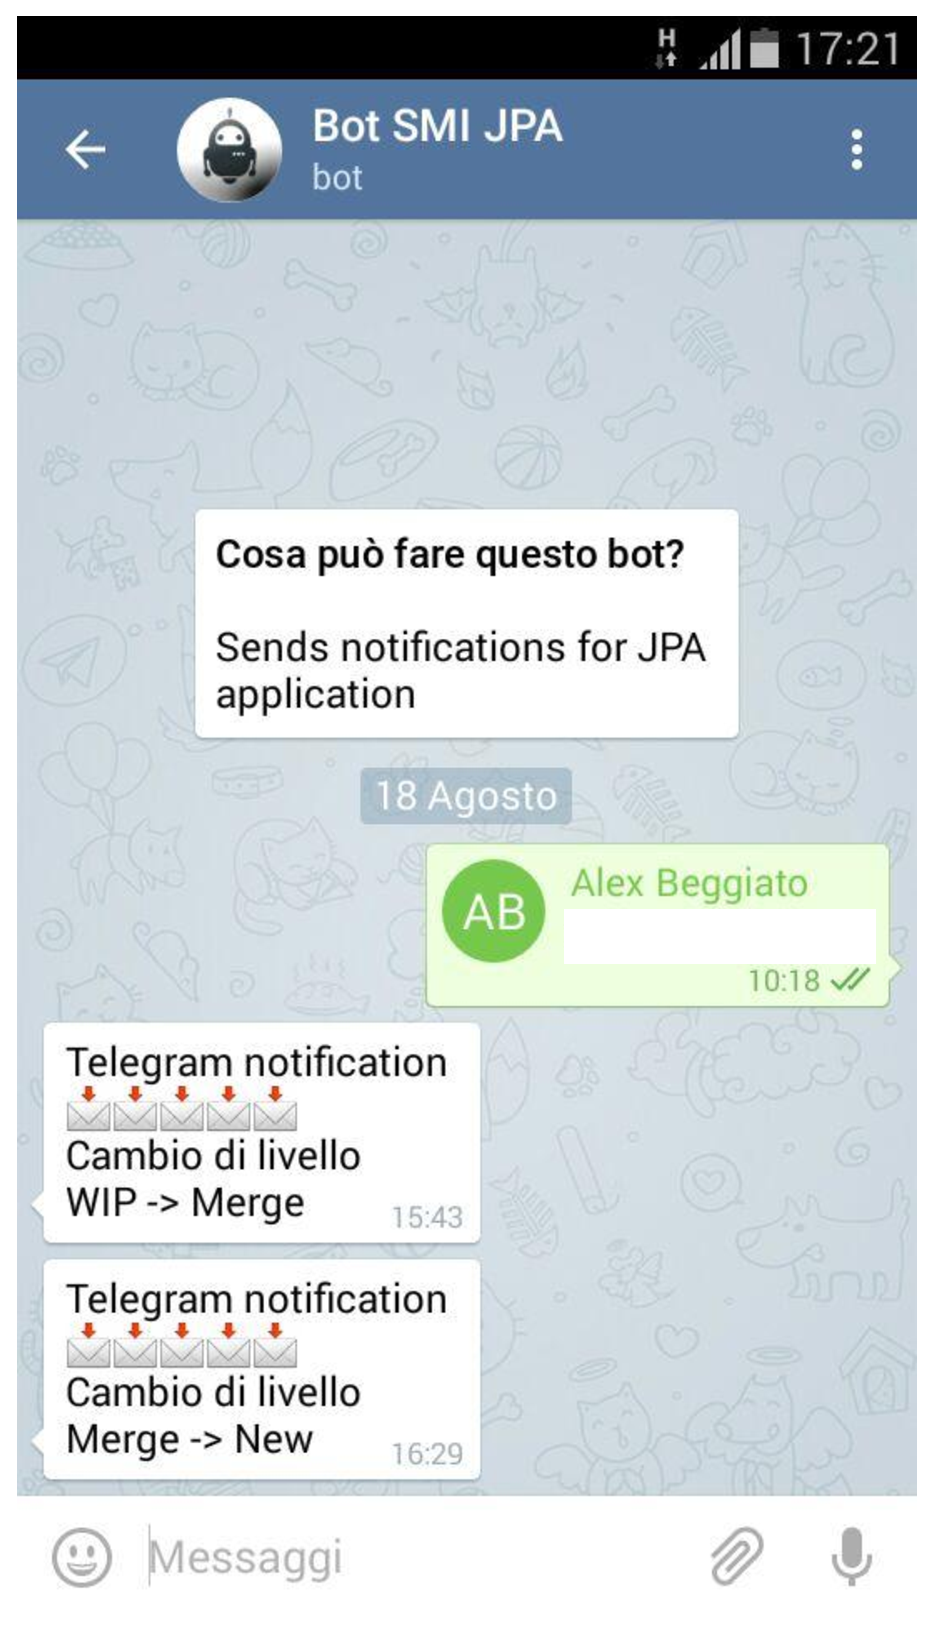
\includegraphics[width=.5\columnwidth]{immagini/telegram-screen}
\caption{Ricezione di notifiche da SmiJpaBot}
\label{fig:screen-telegram}%
\end{figure}

\paragraph{Sviluppi ulteriori con Telegram Bot} \mbox{} \\

L'ultimo sviluppo nell'attività di stage ha portato a implementare ulteriori
funzionalità riguardanti i Telegram Bot:

\begin{itemize}
\item realizzazione di un modulo in cui viene spiegato come creare un Telegram
  Bot ed in seguito collegarlo a JPA;
\item gestione dei contatti telefonici di un utente e di un'eventuale
  associazione del proprio numero ad un account Telegram;
\item prototipazione di invio e ricezione documenti tramite Bot.
\end{itemize}

\begin{tabular}{| c | p{10cm} |}

\hline
\textbf{Requisito} & \textbf{Descrizione} \\
\hline
RF1Obb &
JPA deve disporre di un modulo in cui viene spiegato come creare un Telegram
  Bot. \\
\hline
RF2Des &
JPA deve poter inviare e ricevere documenti tramite un Telegram Bot. \\
\hline
RF2.1Des &
JPA deve poter ricevere documenti tramite un Telegram Bot. \\
\hline
RF2.2Des &
JPA deve poter inviare documenti tramite un Telegram Bot. \\
\hline
RF2.3Des &
JPA deve poter inoltrare documenti tramite un Telegram Bot. \\
\hline
RF3Obb &
JPA deve permettere la gestione del contatto telefonico di un utente. \\
\hline
RF3.1Obb &
JPA deve permettere l'inserimento del numero di telefono di un utente. \\
\hline
RF3.2Obb &
JPA deve permettere la modifica del numero di telefono di un utente. \\
\hline
RF3.3Obb &
JPA deve permettere la disassociazione di un utente dall'account Telegram a
  cui è collegato. \\
\hline
RF4Des &
JPA deve poter ricevere un codice identificativo per un Telegram Bot al fine
  di utilizzarlo per l'invio di notifiche. \\
\hline
RNF1Obb &
Le istruzioni per la creazione ed associazione di Telegram Bot devono essere
  sia in lingua italiana che in inglese.
\\
\hline
RNF2Obb &
Le norme di sviluppo adottate devono essere rispettate.
\\
\hline
RNF3Des &
Le raccomandazioni di sviluppo adottate devono essere rispettate.
\\
\hline
\end{tabular}
\captionof{table}{Requisiti individuati per gli obiettivi dell'ottava
  settimana}
\label{tab:requisiti-prototipo}

%******************************************************************************
%******************************************************************************
%******************************************************************************
%******************************************************************************
%******************************************************************************

\subsection{Progettazione}\label{sec:prog-progettazione}

\paragraph{Checklist} \mbox{} \\

La progettazione per il modulo di checklist è proceduta sviluppando le norme
precedentemente elencate.

Siccome la funzionalità di avere checklist è nuova in JPA ed è indipendente
dal resto del programma, ho introdotto un'area esclusivamente per questa
avente i moduli di gestione template e gestione istanze.

Oltre a questi due moduli, ho deciso di realizzare quattro
\glosspl{direttiva} in modo tale da creare delle componenti riusabili nei
moduli dell'area Checklist e delle altre aree presenti in JPA:

\begin{enumerate}
\item \texttt{cl-tmpl}, usata per template di checklist. Ha dipendenza verso
  \texttt{cl-row};
\item \texttt{cl-row}, \gloss{direttiva} rappresentante una riga di checklist
  appartenente a un template;
\item \texttt{cl-instances}, usata per rappresentare istanze di checklist: ha
  dipendenze verso \texttt{cl-tmpl}, poichè questa direttiva fornisce anche le
  funzionalità di importazione e creazione da template;
\item \texttt{inst-rows}, usata per rappresentare le righe di un'istanza di
  checklist. Ha dipendenze verso \texttt{cl-instances} e \texttt{cl-tmpl}
  poichè al suo interno contiene righe sia di istanze che di template di
  checklist.
\end{enumerate}

\begin{figure}[H]%
\centering
\includegraphics[width=\columnwidth]{immagini/cl-plugin}
\caption{Diagramma delle classi per l'area Checklist}
\label{fig:checklist-cd}%
\end{figure}

Queste \glosspl{direttiva} sono in seguito state utilizzate nei moduli
dell'area Scrum, collegando task appartenenti a quest'area con istanze di
checklist.

\paragraph{Burn-down chart} \mbox{} \\

Per lo sviluppo del burn-down chart erano richieste principalmente tre
modifiche architetturali al \FREND:

\begin{enumerate}
\item la modifica della classe rappresentante l'entità ``livello'', in modo 
  tale da prevedere che a questo potessero essere associate:
  \begin{itemize}
  \item una percentuale di completamento per il task una volta che questo
    riesce a raggiungere un certo livello;
  \item il fatto di poter essere proporzionale ad una checklist\footnote{Solo
    un livello tra tutti può essere proporzionale}.
  \end{itemize}
\item l'inclusione della direttiva \texttt{angular-google-chart} per poter
  usare le \textbf{Google Chart \gloss{api}} in JPA;
\item l'introduzione di una \gloss{direttiva} riusabile nei vari moduli in cui
  si vuole dare la possibilità di selezionare uno sprint e visualizzare un
  burn-down chart per questo.
\end{enumerate}

\paragraph{Strumenti di \emph{Inspection}} \mbox{} \\

Ho inserito i nuovi strumenti di \emph{Inspection} in un modulo dedicato
appositamente per contenerli, \gloss{kpi}.

Tale modulo è stato inserito nell'area Scrum e permette di visualizzare
solamente alcuni dei vari grafici tramite semplici modifiche alla View.

\paragraph{Avvio istanza di processo} \mbox{} \\

Con l'avvio di istanza di processo è stato creato il primo \emph{Angular
Service} nella parte di \FREND{}, ovvero \texttt{ProcessService}, contenuto
nella collezione \texttt{processInstancesServices}.

Tale componente offre metodi per recuperare i possibili processi avviabili da
task e sprint, fattorizzando il codice sparso nei vari Controller dell'area
Scrum.

Oltre a questo, ho applicato modifiche minori a JPADb per poter salvare
collegamenti tra istanze di processi e elementi Scrum.

\begin{figure}[H]%
\centering
\includegraphics[width=.8\columnwidth]{immagini/ProcessService}
\caption{Diagramma delle classi per le funzionalità di avvio istanza}
\label{fig:inst-start-cd}%
\end{figure}

\paragraph{Realizzazione di \gloss{api} per l'area Scrum} \mbox{} \\

Dopo aver progettato la parte che collega l'area Scrum verso quella di gestione
processi, ho realizzato delle \gloss{api} che permettessero lo stesso
collegamento nel verso opposto, ovvero dai processi verso l'area Scrum.

Lo sforzo progettuale che ho impiegato è stato sostanzialmente nullo, poichè ho
semplicemente aggiunto al package JPAUtil una classe, nella quale venivano
forniti dei metodi statici che implementassero le operazioni richieste.

\paragraph{Funzionalità di notifica} \mbox{} \\

Lo sviluppo delle funzionalità di notifica ha richiesto di progettare
l'architettura relativa a questa parte di JPA in modo tale che questa sia
facilmente estensibile:

\begin{itemize}
\item a differenza delle checklist e del burn-down chart, le notifiche possono
  avere ulteriori sviluppi molto più frequentemente, come l'aggiunta di un
  evento da seguire o il supporto a un nuovo mezzo di comunicazione;
\item l'algoritmo che interpreta il codice pensato per la scrittura di corpo e
  titolo di notifiche potrebbe essere reso più efficiente o modificato per
  cambio di codifica di tali testi.
\end{itemize}

L'architettura progettata (fig. \ref{fig:arch-notif}) prevede quindi le
seguenti componenti:

\begin{itemize}
\item \texttt{Notification}, una classe che rappresenta messaggi;
\item \texttt{NotificationBuilder}, una classe che rappresenta un costruttore
  di notifiche;
\item \texttt{NotificationDirector}, una classe che organizza la costruzione
  di notifiche. Insieme a \texttt{NotificationBuilder} realizza il
  \gloss{design-pattern} \textbf{Builder};
\item \texttt{Action}, una classe che al suo interno ha i parametri relativi
  ad un particolare evento;
\item \texttt{Decoder}, una classe in cui viene racchiuso l'algoritmo di
  decodifica. Fa uso del \gloss{design-pattern} \textbf{Template Method};
\item \texttt{DecoderFactory}, una classe che istanzia degli oggetti di tipo
  \texttt{Decoder}. Realizza il \gloss{design-pattern} \textbf{Factory Method}.
\end{itemize}

\texttt{Notification} è una classe astratta che possiede un oggetto, un corpo,
un mittente e dei destinatari. In particolare offre il metodo astratto
\texttt{send()}, implementato dalle sottoclassi per poter inviare il
messaggio\footnote{Realizza il \gloss{design-pattern} \textbf{Strategy}}. Da
questa classe al termine dello stage derivavano le classi
\texttt{internalmail.InternalMail} e
\texttt{telegram.TelegramMessage}\footnote{Come per il relativo
\emph{builder}, al termine di tale sviluppo questa classe era assente}, che
rappresentano rispettivamente una notifica da mandare via mail interna in JPA
e via messaggio da Telegram Bot.

\texttt{NotificationBuilder} è una classe astratta che mantiene un riferimento
a un oggetto di tipo \texttt{Notification}, visibile alle sottoclassi. Grazie
a dei metodi \emph{setter} è possibile costruire un
\texttt{NotificationBuilder} specificando solamente le parti necessarie di
questo ed evitando in questo modo il fenomeno chiamato \gloss{telescoping}.

Una volta istanziato un costruttore di notifiche, si lascia la possibilità ad
un oggetto di tipo \texttt{NotificationDirector} di eseguire dei metodi
implementati dalle sottoclassi per specificare come scrivere i vari elementi
di una notifica. In questo modo, la logica di costruzione del messaggio viene
spostata interamente in \texttt{NotificationBuilder}.

Attualmente vi sono due sottoclassi di questo \emph{builder}, ovvero
\texttt{telegram.TelegramBuilder} e \texttt{internalmail.InternalMailBuilder},
che costruiscono rispettivamente notifiche da mandare via Telegram e mail
interna.

All'interno di \texttt{NotificationDirector} vi è la ``ricetta'' per costruire
una notifica per mezzo delle operazioni offerte da un oggetto di tipo
\texttt{NotificationBuilder}.

\texttt{Decoder} incapsula l'algoritmo di decodifica dei testi di oggetto e
corpo delle notifiche. Questa classe realizza il \gloss{design-pattern}
\textbf{Template Method} poichè dichiara un metodo, \texttt{getKeywords()}, la
cui implementazione è responsabilità delle sottoclassi e che viene usato
dall'operazione pubblica \texttt{decode(text : String)}.

In base all'evento che ha scatenato la notifica, \texttt{DecoderFactory}
istanzia un \texttt{Decoder} appropriato che provvederà ad eseguire una
decodifica semplice o ciclica, a seconda che la notifica legata a un dato
evento consenta la presenza di cicli.

L'intera progettazione architetturale per questa parte di JPA è stata raccolta
in una specifica tecnica consegnata a Sanmarco Informatica, in cui vengono
indicati anche:

\begin{itemize}
\item come aggiungere eventi o tipi di notifiche;
\item eventuali migliorie di efficienza (e.g. cambiare i
  \texttt{NotificationBuilder} in classi \texttt{Runnable}, ovvero eseguibili
  concorrentemente);
\item avvertimenti, nel caso debba essere fornita obbligatoriamente
  un'implementazione non vuota ad alcuni metodi astratti di superclassi.
\end{itemize}

\begin{landscape}
\begin{figure}%
\centering
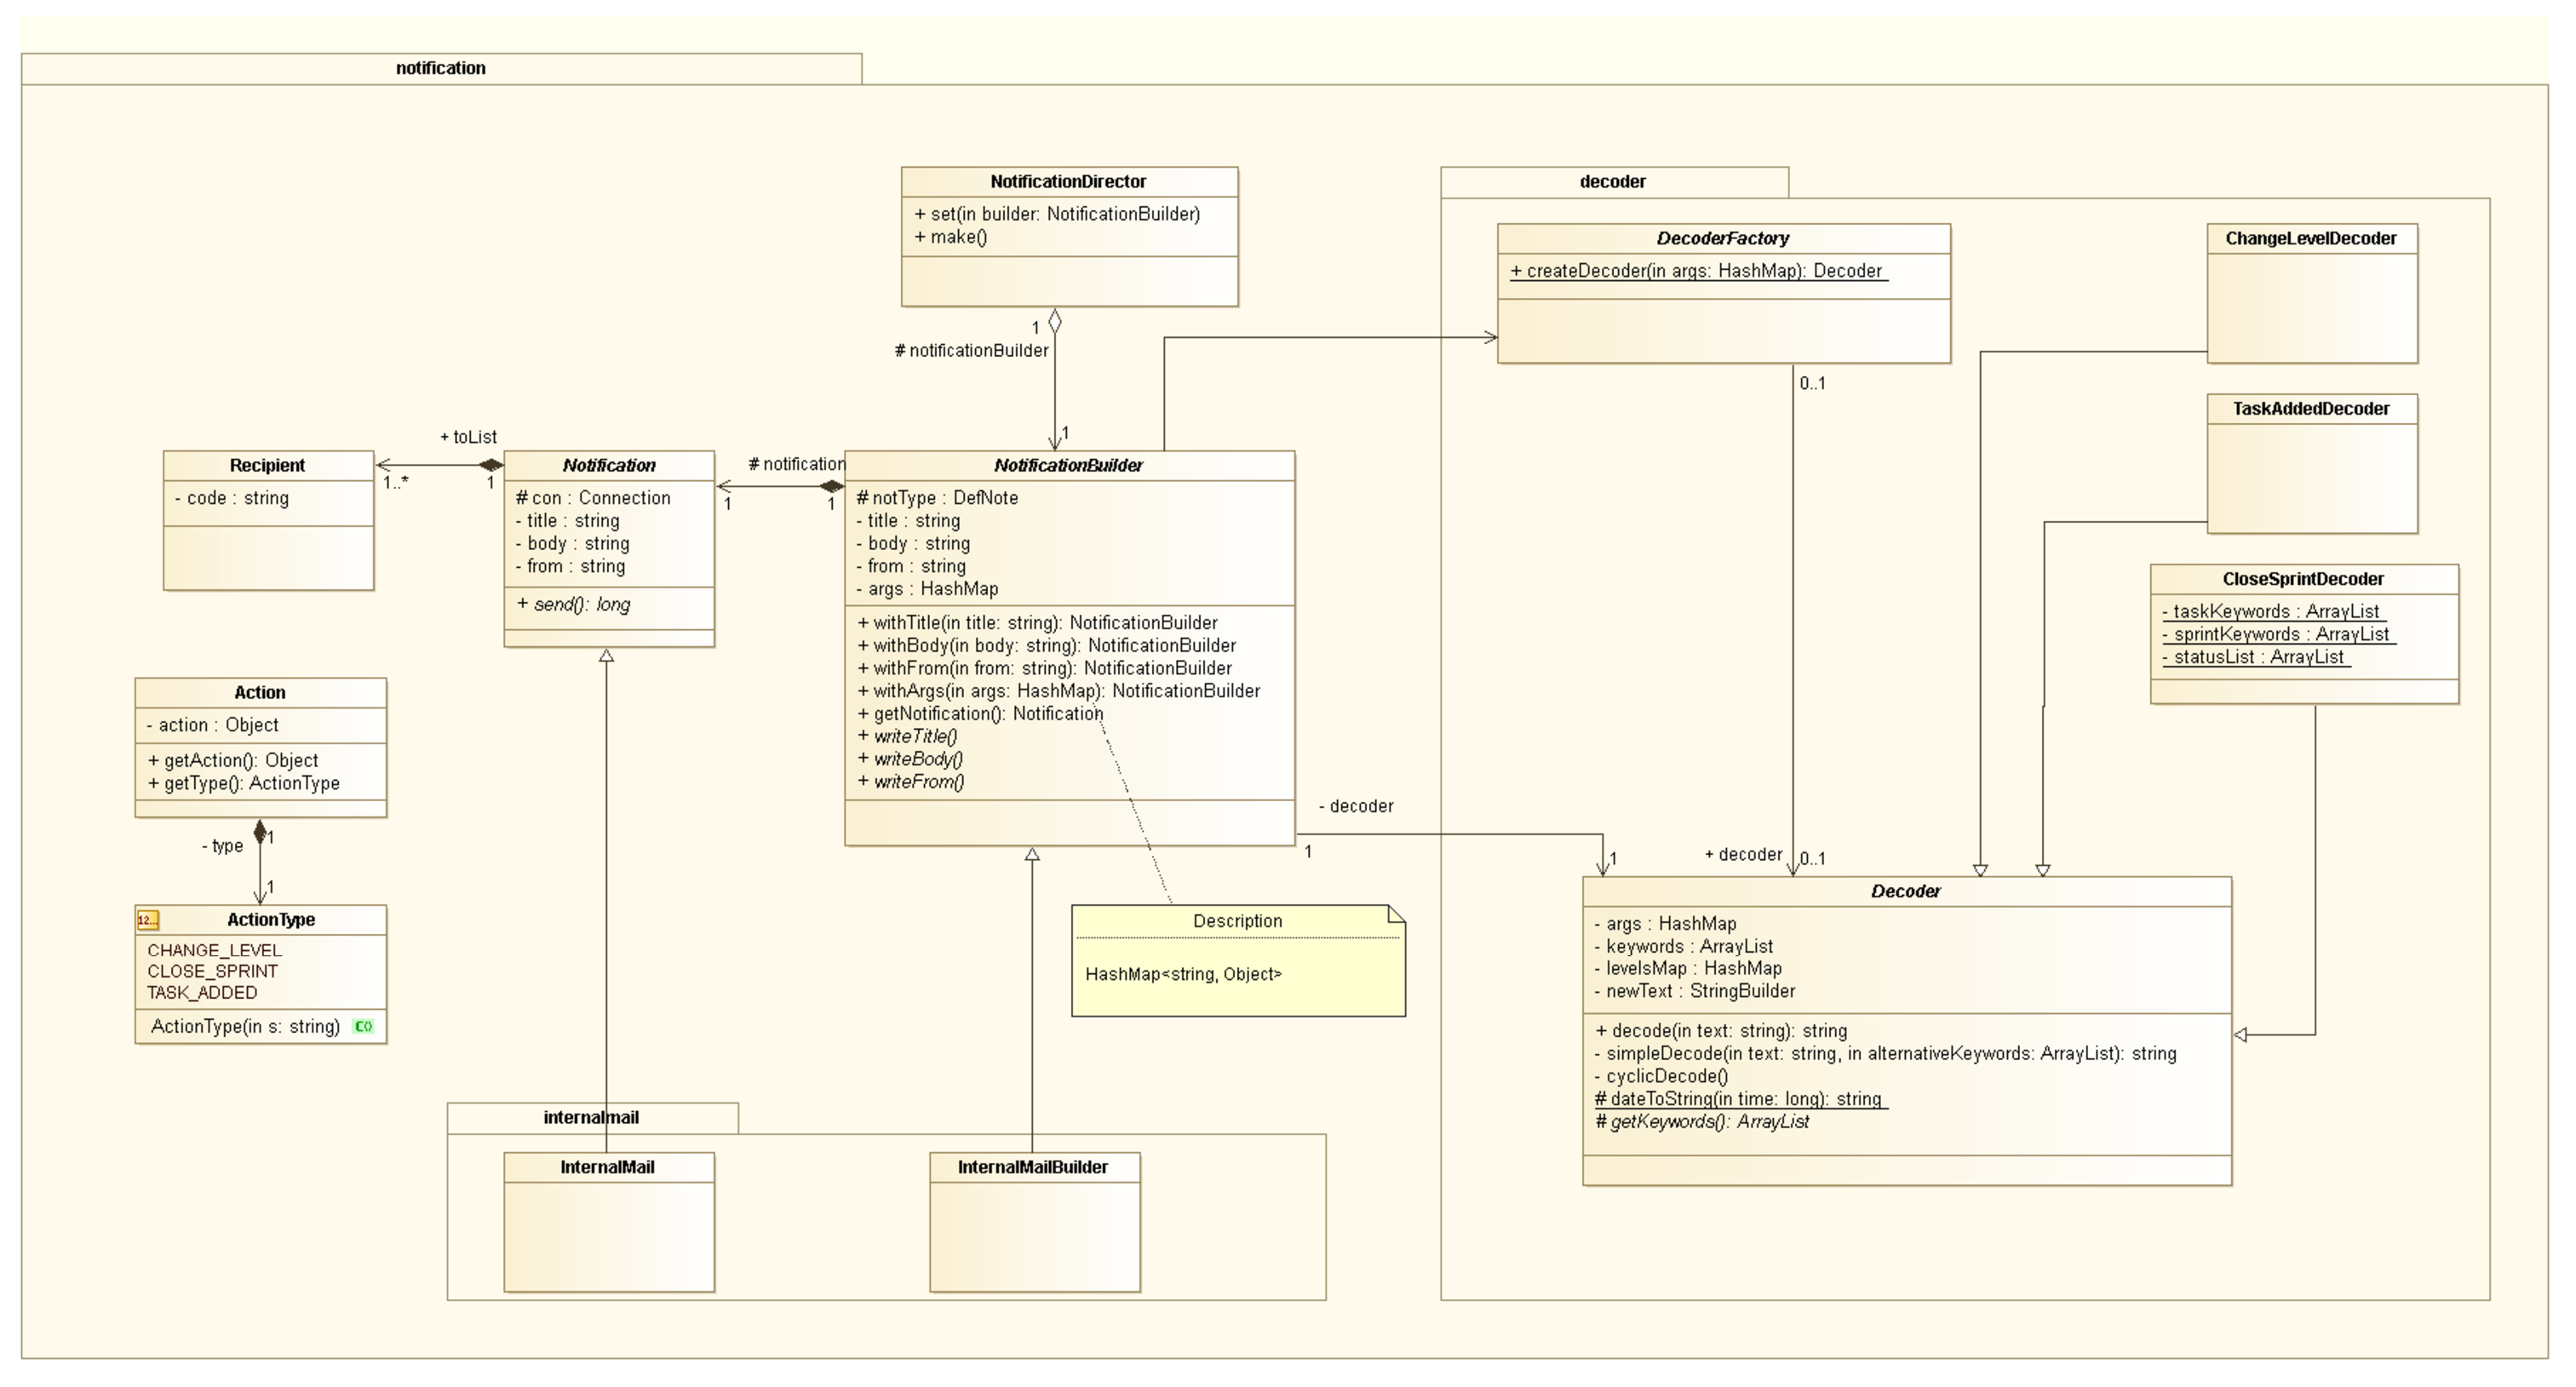
\includegraphics[width=\columnwidth]{immagini/notif-class_diagram}
\caption{Diagramma delle classi per le funzionalità di notifica}
\label{fig:arch-notif}%
\end{figure}
\end{landscape}

\paragraph{Collegamento al forum} \mbox{} \\

Per quanto riguarda il \BKEND{}, ho aggiunto delle operazioni all'area Scrum
che causano una dipendenza verso l'area Forum.

Nel \FREND{} ho invece introdotto due servizi nella collezione
\texttt{forumServices}:

\begin{enumerate}
\item \texttt{TaskForum}: fornisce metodi di utilità per il collegamento tra
  task Scrum e area Forum;
\item \texttt{SprintForum}: fornisce metodi di utilità per il collegamento tra
  sprint e area Forum.
\end{enumerate}

\paragraph{Notifiche via Telegram} \mbox{} \\

Tale tipo di notifica, sviluppato come obiettivo aggiuntivo, ha messo alla
prova l'estensibilità dell'architettura realizzata per le funzionalità di
notifica.

Prima dell'implementazione delle notifiche via Telegram, avevo modificato
l'architettura solamente con aggiungendo di eventi. L'insieme dei mezzi di
comunicazione per inviare una notifica si limitava infatti al semplice invio
di una mail interna in JPA.

Dopo aver confrontato la possibilità di inviare messaggi con un Telegram Bot o
con le \gloss{api} ed un account legato a persona reale, ho preferito la
soluzione che prevedeva l'uso di un Bot:

\begin{itemize}
\item i Bot sono strumenti sviluppati e pensati appositamente per lo
  svolgimento di compiti automatici;
\item sebbene i Bot siano stati introdotti molto recentemente, la
  documentazione fornita da Telegram è ottima e dopo un breve periodo di
  prototipazione si può notare che il funzionamento di questi rispetta
  fedelmente le attese.
\end{itemize}

Seguendo le istruzioni nella Specifica Tecnica realizzata per tale frazione
dell'architettura, ho esteso JPA arrivando a comprendere anche le notifiche
via Telegram.

Anche per la parte relativa alle funzionalità di notifica ho progettato la
collezione \texttt{followServices}, un insieme di \emph{Angular Service} che
potesse raccogliere i servizi relativi alle funzionalità di
notifica\footnote{Le funzionalità relative ai task non sono state raccolte in
un \emph{Angular Service} in accordo con il tutor aziendale}, in cui sono
presenti \texttt{SprintFollowers} e \texttt{CommonFollow}.

\texttt{SprintFollowers} è un servizio che contiene le seguenti operazioni
relative agli sprint:

\begin{itemize}
\item \texttt{getFollowers()}: metodo con il quale è possibile recuperare
  tutti i seguaci degli eventi di uno sprint;
\item \texttt{setFollow()}: metodo con il quale richiedere di seguire un
  evento sprint con un certo tipo di notifica.
\end{itemize}

\texttt{CommonFollow} è un servizio che contiene le seguenti operazioni
relative agli sprint:

\begin{itemize}
\item \texttt{getActionsMap()}: metodo con il quale è possibile recuperare i
  possibili eventi che è possibile seguire e per quali elementi Scrum sono
  disponibili;
\item \texttt{getNotificationTypes()}: metodo con il quale è possibile
  recuperare i tipi di notifica disponibili.
\end{itemize}

\paragraph{Sviluppi ulteriori con Telegram Bot} \mbox{} \\

In primo luogo, ho aggiunto funzionalità per gestire il contatto telefonico di
un utente e la sua associazione a Telegram.

Ciò ha comportato semplicemente modifiche leggere alla struttura di alcune
tabelle in JPADb e al modulo di gestione del proprio profilo utente.

Gli altri sviluppi hanno riguardato i Telegram Bot: un modulo di istruzioni per
la creazione di un Bot e l'associazione di questo a JPA e la prototipazione
per lo scambio di documenti via Telegram.

Per il primo, ho aggiunto un nuovo modulo all'area di configurazione di
JPA: concordemente con il tutor aziendale, ho deciso di sviluppare questo
modulo diversamente dagli altri e di introdurre un'eccezione alla regola di
usare delle label per ogni frase presente nella View HTML.

Questa eccezione è dovuta al fatto che in questa pagina è presente molto testo,
includibile più facilmente introducendo nell'architettura di questo modulo due
\emph{template} (parti di pagina) HTML, uno in italiano ed uno in inglese.

Per il secondo, ho introdotto in JPA una classe
\texttt{http.HTTPRequestSender} con al suo interno delle \gloss{api} per
effettuare delle chiamate \gloss{rest} di tipo GET e POST. Successivamente, da
questa classe ho fatto derivare \texttt{http.TelegramHTTPRequestSender} in modo
tale da avere delle \gloss{api} che effettuassero delle chiamate per il Bot
associato a JPA.

A questo punto, ho aggiunto le operazioni di scambio documenti alle classi
\texttt{ScTelegram} e \texttt{ScTelegramUtil}.

%******************************************************************************
%******************************************************************************
%******************************************************************************
%******************************************************************************
%******************************************************************************

\subsection{Codifica}\label{sec:prog-codifica}

In questa sezione vengono esposti i punti salienti incontrati durante
l'attività di codifica. Prima di mostrarli, viene brevemente esposta la
procedura con la quale avveniva questa attività:

\begin{itemize}
\item le tabelle di JPADb vengono modificate e i relativi script vengono
  immediatamente integrati al ramo principale di SVN;
\item le modifiche al \BKEND{} vengono codificate con il seguente ordine per le
  operazioni \gloss{crud}: \emph{Read}, \emph{Create}, \emph{Update},
  \emph{Delete};
\item il \FREND{} veniva invece sviluppato una volta che la parte di \BKEND{}
  veniva ritenuta stabile.
\end{itemize}

\paragraph{Checklist} \mbox{} \\

Sebbene la complessità dell'implementazione del modulo di checklist non fosse
di per sè complicata da un punto di vista algoritmico o architetturale, nelle
prime settimane di stage ho riscontrato difficoltà dovute all'inesperienza che
hanno causato i ritardi evidenziati in tabella \ref{tab:deviazioni}.

I principali ostacoli che ho riscontrato sono stati l'adeguarsi ad un nuovo
insieme di norme e far propri alcuni aspetti tipici della programmazione
funzionale ed asincrona.

\paragraph{Burn-down chart} \mbox{} \\

A differenza dello sviluppo delle checklist, l'implementazione della
\gloss{direttiva} per il burn-down chart e dei relativi servizi offerti dal
\BKEND{} non è stata banale.

Questo è dovuto a diversi fattori:

\begin{itemize}
\item come detto in precedenza, l'inclusione della \gloss{direttiva}
  \texttt{angular-google-chart} ha ristretto alcune funzionalità offerte dalle
  \textbf{Google Chart \gloss{api}};
\item il burn-down chart doveva ignorare i sabati e le domeniche, sia nella
  parte di \BKEND{} che in quella di \FREND{};
\item i dati dovevano essere ricavati da dei log, quindi prima di riuscire ad
  effettuare tutte le computazioni necessarie era necessario preparare i dati
  in ingresso;
\item l'insieme di livelli possibili per JPA non è noto a priori;
\item l'implementazione del requisito desiderabile da me proposto, ovvero il
  gradiente di colorazione per i livelli, si è rivelato più difficile di
  quanto stimato inizialmente;
\item vi era la necessità di trattare con attenzione l'eventuale livello il
  cui avanzamento può essere ritenuto proporzionale al completamento di una
  checklist.
\end{itemize}

\paragraph{Strumenti di \emph{Inspection}} \mbox{} \\

La codifica per gli strumenti di \emph{Inspection} è consistita nel riuscire
ad elaborare i dati già presenti per il burn-down chart per adattarli agli
altri tipi di grafico.

Ho applicato tutte le modifiche alla parte di \FREND{}, poichè i dati
forniti dal \BKEND{} erano sufficientemente completi per poter essere riusati
per più scopi.

Per lo sviluppo del documento di descrizione dei vari strumenti mi sono
ispirato al libro \emph{Design Patterns: Elements of Reusable Object-Oriented
Software} (Gamma, Helm, Johnson, Vlissides).

Come nel testo sopra citato ciascun \gloss{design-pattern} ha lo stesso
insieme di caratteristiche spiegate, nel documento da me realizzato per ogni
strumento di \emph{Inspection} sono indicati:

\begin{itemize}
\item il suo nome;
\item eventuali sinonimi o termini con cui lo strumento è conosciuto;
\item il suo scopo, ovvero una breve risposta alla domanda ``\emph{A cosa
  serve questo strumento?}'';
\item la sua rappresentazione grafica;
\item una motivazione che spiega più approfonditamente perchè lo strumento è
  adatto per lo scopo sopra dichiarato;
\item uno scenario in cui tale strumento è utilizzabile;
\item le misurazioni (in termini di indici \gloss{kpi}) che si possono
  ottenere tramite l'uso dello strumento;
\item eventuali varianti disponibili su JPA.
\end{itemize}

\paragraph{Avvio istanza di processo} \mbox{} \\

Non ho trovato particolari difficoltà per tale sviluppo, se non il fatto che
il primo \emph{Angular Service} è stato introdotto in questa occasione.

Dopo aver realizzato la funzionalità senza l'utilizzo di un \emph{Service}, ho
creato un ramo di sviluppo su \textbf{git} in cui ho spostato in
\texttt{ProcessService} la \emph{business logic} presente nei Controller.

A seguito dell'approvazione del tutor aziendale, ho integrato tale ramo a
quello principale nel \gloss{repository} che ho utilizzato per gestire lo
sviluppo del \FREND{}.

\paragraph{Funzionalità di notifica} \mbox{} \\

Per tale sviluppo era previsto che io realizzassi un linguaggio di
trasformazione simile all'XSLT (\emph{eXtensible Stylesheet Language
Transformations}), in cui è possibile sostituire parti di testo con parametri
legati agli eventi per i quali è stata richiesta la ricezione di notifiche.

Questa non era l'unica difficoltà legata a questo sviluppo:

\begin{itemize}
\item dal momento che l'architettura era complessa, ho utilizzato dei
  \gloss{design-pattern}. La loro implementazione è risultata più facile
  ispirandomi a degli
  esempi\footnote{\url{https://github.com/snate/design_pattern}} che
  avevo realizzato durante il terzo anno di università ed adattandoli alle
  esigenze specifiche del problema incontrato;
\item oltre alla scrittura del testo della notifica, vi era una complessità
  algoritmica non banale anche nel recupero dei contatti da notificare e del
  modo in cui notificare ciascuno di essi.
\end{itemize}

Oltre alle difficoltà sopra elencate, un obiettivo che mi sono posto è non
superare l'annidamento di tre cicli per l'invio di ciascuna notifica, in modo
da rendere la funzionalità scalabile.

Al contempo, il problema presentava le seguenti facilitazioni:

\begin{itemize}
\item l'algoritmo di decodifica non ha l'obbligo di interpretare cicli
  innestati;
\item l'algoritmo di decodifica non garantisce un output corretto a seguito di
  un input testuale malformato;
\item l'algoritmo che invia una mail interna in JPA è stato ricopiato da una
  funzione già esistente.
\end{itemize}

\paragraph{Collegamento al forum} \mbox{} \\

Per le funzionalità di collegamento al forum non ho incontrato particolari
difficoltà durante l'attività di codifica.

\paragraph{Notifiche via Telegram} \mbox{} \\

Prima di poter cominciare a sviluppare le funzionalità di notifica via
Telegram, ho creato un Telegram Bot di nome JPASmiBot.

Una volta generato il Bot, ho proceduto a capire come poter utilizzare al
meglio le sue capacità. I Telegram Bot possono ricevere in due modi i messaggi
che gli utenti Telegram inviano loro, ovvero secondo il \emph{push} o il
\emph{pull} model.

Si è deciso di ricevere messaggi per il Bot con il \emph{pull} model, siccome
per l'altra modalità era necessario fornire l'URL al quale inviare chiamate
\gloss{rest} provenienti da Telegram e, dialogando con il tutor aziendale, è
stato deciso di non renderlo disponibile all'esterno.

Dopo un'analisi delle \gloss{api} disponibili per i Telegram Bot, si è deciso
di richiedere l'associazione del proprio contatto Telegram inviando il proprio
contatto telefonico come messaggio.

Per la conversione degli oggetti \gloss{json} che venivano ricevuti all'arrivo
degli aggiornamenti, è stata utilizzata \textbf{Gson}, una libreria Java di
Google.

Grazie a questa libreria, è possibile trasformare facilmente gli oggetti
\gloss{json} creando delle classi che abbiano le stesse proprietà di questi (e
viceversa) con le funzioni \texttt{toJson()} e \texttt{fromJson()}. Gson ha i
suoi punti di forza nell'efficienza e nel riuscire a fornire supporto ai
Generics di Java.

Ho proseguito con la codifica come descritto nella sezione
\ref{sec:prog-progettazione}, estendendo l'architettura ed implementando
l'invio di messaggi a partire dalle \gloss{api} Telegram.

Una caratteristica interessante dell'architettura è vedere come il fatto di
aver inserito un \emph{builder} sia risultato determinante una volta arrivati
all'aggiunta di un tipo diverso di modalità di notifica, non dovendo in alcun
modo modificare la decodifica dei testi dei messaggi di notifica.

Durante l'attività di stage, i messaggi su Telegram potevano essere costituiti
da semplice testo, al limite accompagnato da emoji\footnote{Ciò non è più
vero: dal 7 settembre è stato aggiunto supporto di base (con possibilità di
usare il grassetto, il corsivo e l'inserimento di link) per il
\gloss{markdown}}. Per questo motivo, la separazione tra titolo e corpo di una
notifica è stata realizzata inserendo, tramite il processo di costruzione
notifica, una riga con cinque emoji rappresentanti una busta tra le due parti
di messaggio (come è possibile vedere in figura \ref{fig:screen-telegram}).

\paragraph{Sviluppi ulteriori con Telegram Bot} \mbox{} \\

Lo stage si è concluso sviluppando delle funzionalità relative ai Telegram Bot.

Il modulo di guida per la creazione di un proprio Bot non è stato
particolarmente complicato da realizzare, poichè ricalcava quanto già fatto
con i Manuali Utente.

Ho riscontrato maggiori problemi per lo scambio di documenti via Telegram: ciò
è dovuto al fatto che la ricezione di file è al momento supportata solamente
per gli account ``reali'' e non per i Bot.

Tuttavia, al momento sono disponibili le \gloss{api} sia l'invio di un file
presente nel dispositivo locale che l'inoltro di un file ricevuto (anche se da
un Bot), le quali sono state utilizzate per portare a termine l'obiettivo
produttivo fissato.

Per lo sviluppo delle chiamate \gloss{rest} in uscita dal \BKEND{} ho
utilizzato il package \texttt{java.net}.

%******************************************************************************
%******************************************************************************
%******************************************************************************
%******************************************************************************
%******************************************************************************

\subsection{Verifica ed integrazione}\label{sec:prog-verifica}

\paragraph{Verifica} \mbox{} \\

JPA non è inserito in un sistema di \emph{continuous integration} e non dispone
di test automatici che vengono eseguiti ad ogni compilazione dell'applicazione.

Fin dall'inizio dell'attività di stage, ho preso in considerazione l'idea di
impostare un ambiente di test per la parte di \FREND{} che eseguisse verifiche
dinamiche con i \gloss{framework} Jasmine e/o Protractor.

Tuttavia, quest'idea non è stata concretizzata per i seguenti motivi:

\begin{itemize}
\item durante lo stage partivo inesperto nell'uso delle tecnologie per il
  \FREND{} e stavo già investendo buona parte del tempo a mia disposizione per
  apprendere queste. Aggiungendo lo studio dei \gloss{framework} di test, avrei
  rischiato di non imparare ad usare bene nè l'uno nè l'altro insieme di
  tecnologie;
\item l'impiego di tempo lavorativo per la configurazione dell'ambiente di
  test avrebbe potuto mettere a rischio il raggiungimento degli obiettivi
  prestabiliti;
\item l'azienda ripone maggior interesse nello sviluppare un numero elevato di
  funzionalità che nell'automazione dell'attività di verifica. Per questo
  motivo, l'anticipo rispetto al Piano di Lavoro è stato utilizzato per il
  raggiungimento di nuovi obiettivi che andassero ad arricchire le possibilità
  che JPA offriva;
\item per la maggior parte dei casi, la verifica automatica non avrebbe
  garantito un guadagno significativo in termini di efficienza.
\end{itemize}

Come conseguenza di ciò, per la verifica degli incrementi realizzati ho
eseguito prove manuali per verificare la correttezza di \BKEND{} e \FREND{}
con la seguente procedura:

\begin{enumerate}
\item dopo aver (eventualmente) realizzato lo scheletro di un modulo o di una
  \gloss{direttiva} (nella parte di \FREND{}), aggiungere le nuove chiamate
  \gloss{rest} che vengono effettuate verso i \emph{Web services} del \BKEND{}.
  A questo punto:
  \begin{enumerate}
  \item stampare i dati in un formato tale da poter verificare che le
    operazioni vengano eseguite correttamente, se la loro invocazione non
    genera errori;
  \item assegnare un codice univoco alla rilevazione di errori nella chiamata
    di tali metodi.
  \end{enumerate}
\item verificare che ciascuna delle chiamate \gloss{rest} fornisca i risultati
  attesi\footnote{controllando sia lo stato di JPADb che le stampe sul lato
  client}, man mano che queste vengono implementate nel \BKEND{};
\item una volta che è stato verificato che le chiamate \gloss{rest} vadano a
  buon fine, verificare se il comportamento del \FREND{} è corretto andando a
  verificare il soddisfacimento di tutti i requisiti;
\item nel caso in cui uno dei requisiti non sia soddisfatto, modificare il
  \FREND{} e tornare al punto 2, per verificare che le modifiche al \FREND{}
  continuino a passare in modo corretto i parametri ricevuti dal \BKEND{}.
\item L'incremento viene infine presentato al tutor aziendale ed eventuali
  modifiche richieste vengono discusse ed eventualmente applicate e testate;
\item una volta verificati tutti i requisiti e ricevuta l'approvazione dal
  tutor aziendale, veniva svolto un ulteriore collaudo con il quale venivano
  ricavate le immagini per il Manuale Utente;
\item per il Manuale Utente, nei primi periodi di stage è stata svolta
  un'attività di \gloss{walkthrough}, mirata a consolidare uno scheletro da
  riusare per tutti i futuri documenti. In seguito, le verifiche sui documenti
  sono state effettuate esclusivamente sui punti di controllo presenti in
  tabella \ref{tab:inspection}. \\
\end{enumerate}

\begin{figure}[H]%
\centering
\includegraphics[width=1.2\columnwidth]{immagini/verification-flow}
\caption{Flusso dell'attività di verifica}
\label{fig:flow-verification}%
\end{figure}

\begin{tabular}{ | p{4cm} | p{4cm} | p{4cm} | }

\hline
\textbf{Forma} & \textbf{Contenuto} & \textbf{Composizione} \\
\hline
Uso appriopriato delle maiuscole &
Scopo di documento e prodotto adeguati al documento sviluppato &
Uso corretto delle macro  \\
\hline
Accenti mancanti su parole &
Errori nelle didascalie di figure &
Mancata glossarizzazione di termini \\
\hline
Uso corretto dei colori nelle figure &
&
Mancato uso delle parentesi con conseguente omissione dello spazio tra una
macro e la parola successiva \\
\hline
Formato del testo corretto rispetto a quanto dichiarato in introduzione &
&
 \\
\hline
\end{tabular}
\captionof{table}{Punti di controllo per la verifica di documenti}
\label{tab:inspection}

Le attività di verifica devono coprire le varie classi di equivalenza dei
possibili valori in ingresso:

\begin{enumerate}
\item valori \textbf{estremi} dell'intervallo legale, ovvero valori limite per
  i quali JPA deve continuare a funzionare correttamente (e.g. visualizzazione
  di burn-down chart a fine sprint);
\item valori nominali \textbf{interni}, ovvero valori accettabili e non
  estremi (e.g. visualizzazione di burn-down chart in giorni diversi
  dall'inizio o dalla fine);
\item valori \textbf{illegali}, ovvero provando a far fallire il programma nel
  caso di inserimento di valori ritenuti non accettabili (e.g. richiesta di
  visualizzare un burn-down chart per sprint con data di fine anteriore alla
  data di inizio).
\end{enumerate}

\paragraph{Integrazione} \mbox{} \\

Ho integrato gli incrementi sviluppati durante lo stage al ramo principale di
SVN per quanto riguarda il \BKEND{} e JPADb.

Per quanto concerne il \FREND{} invece, solamente le checklist sono state
integrate in JPA durante la mia permanenza a Sanmarco Informatica, nel corso
della quarta settimana.

Ho consegnato tutti gli altri incrementi via Skype con l'intero
\gloss{repository} alla fine dell'attività.

\section{Risultati raggiunti}\label{sec:stage-risultati}

Nel complesso,tutto il lavoro consegnato è stato verificato (e quindi
approvato dal tutor aziendale), compiendo tutti gli sviluppi previsti nella
tabella \ref{tab:piano-di-lavoro}.

Di seguito viene riportato ciò che ho prodotto in JPA per ciascun
obiettivo individuato:

\begin{itemize}
\item \textbf{Checklist:}
  \begin{itemize}
  % MODULO GESTIONE CHECKLIST
  \item Modulo di gestione checklist (fig.
    \ref{fig:gestione-checklist-screen});
    \begin{figure}[H]%
    \centering
    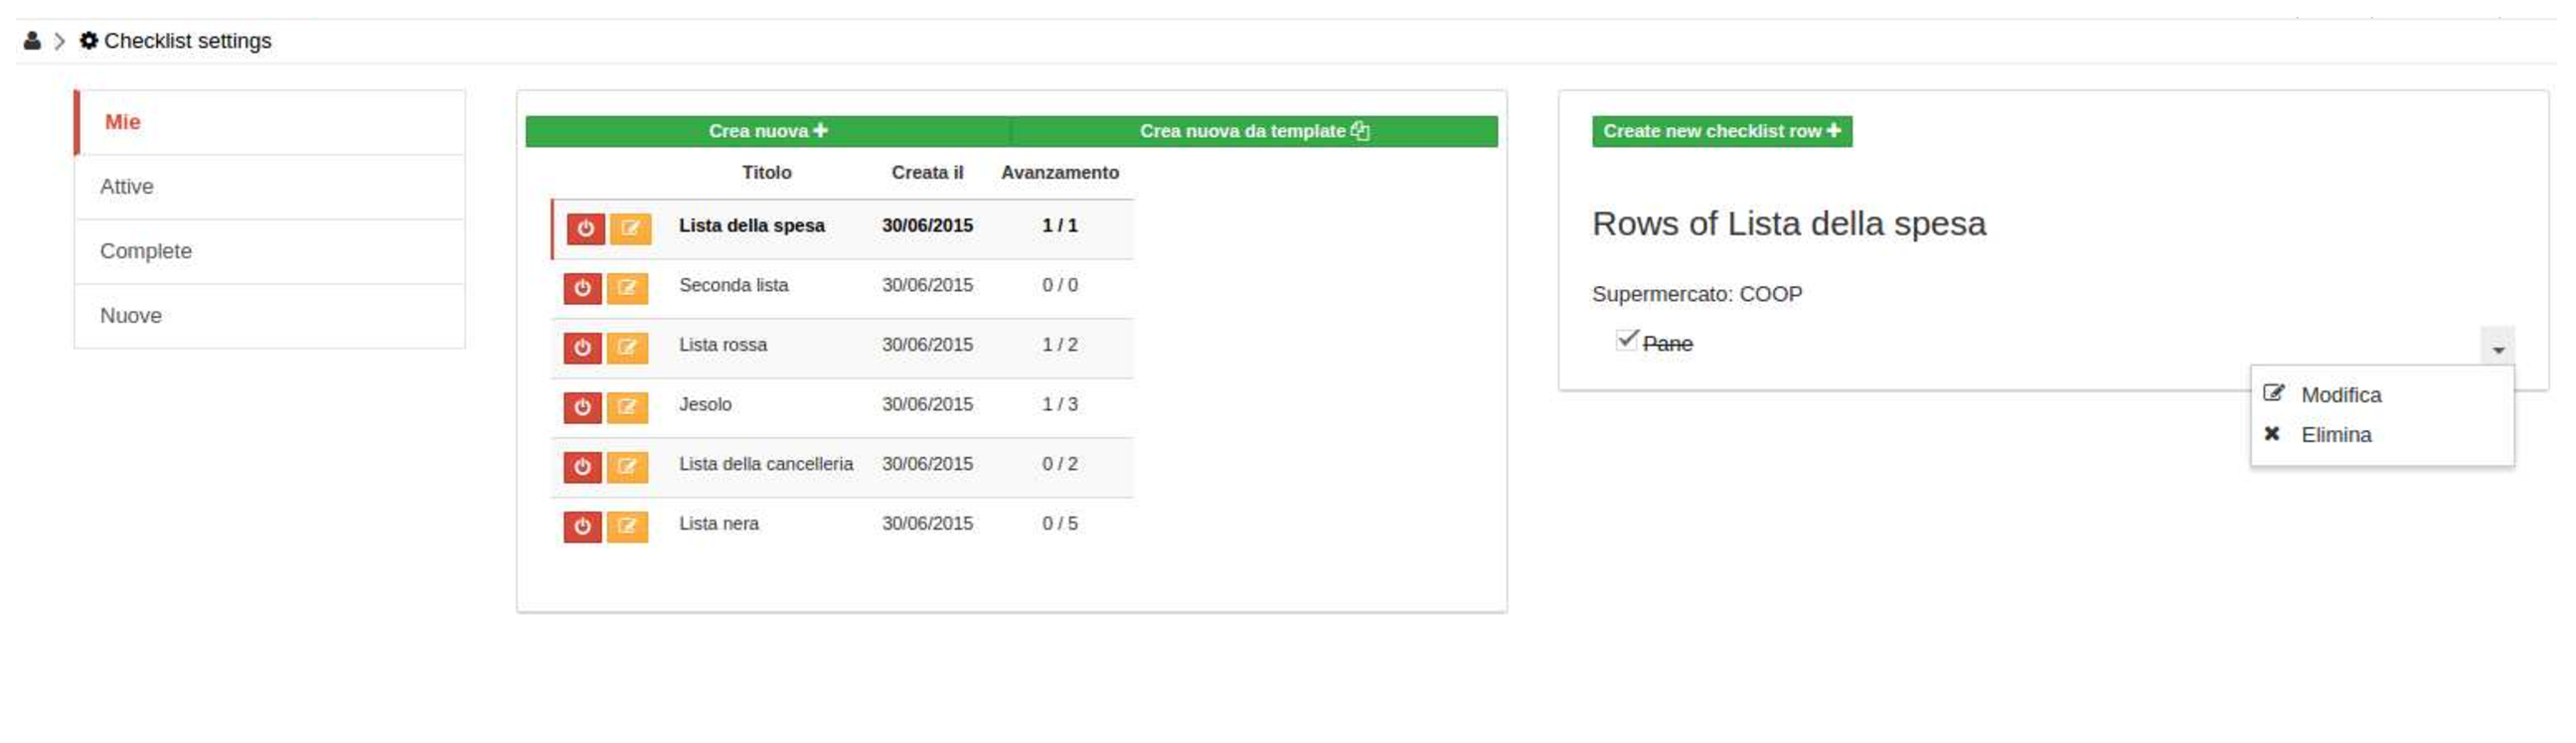
\includegraphics[width=1.2\columnwidth]{immagini/gestioneChecklist}
    \caption{Modulo di gestione checklist}
    \label{fig:gestione-checklist-screen}%
    \end{figure}
  % FINE MODULO GESTIONE CHECKLIST
  % GESTIONE TEMPLATE CL
  \item Modulo di gestione template di checklist (fig.
    \ref{fig:gestione-tmpl-cl});
    \begin{figure}[H]%
    \centering
    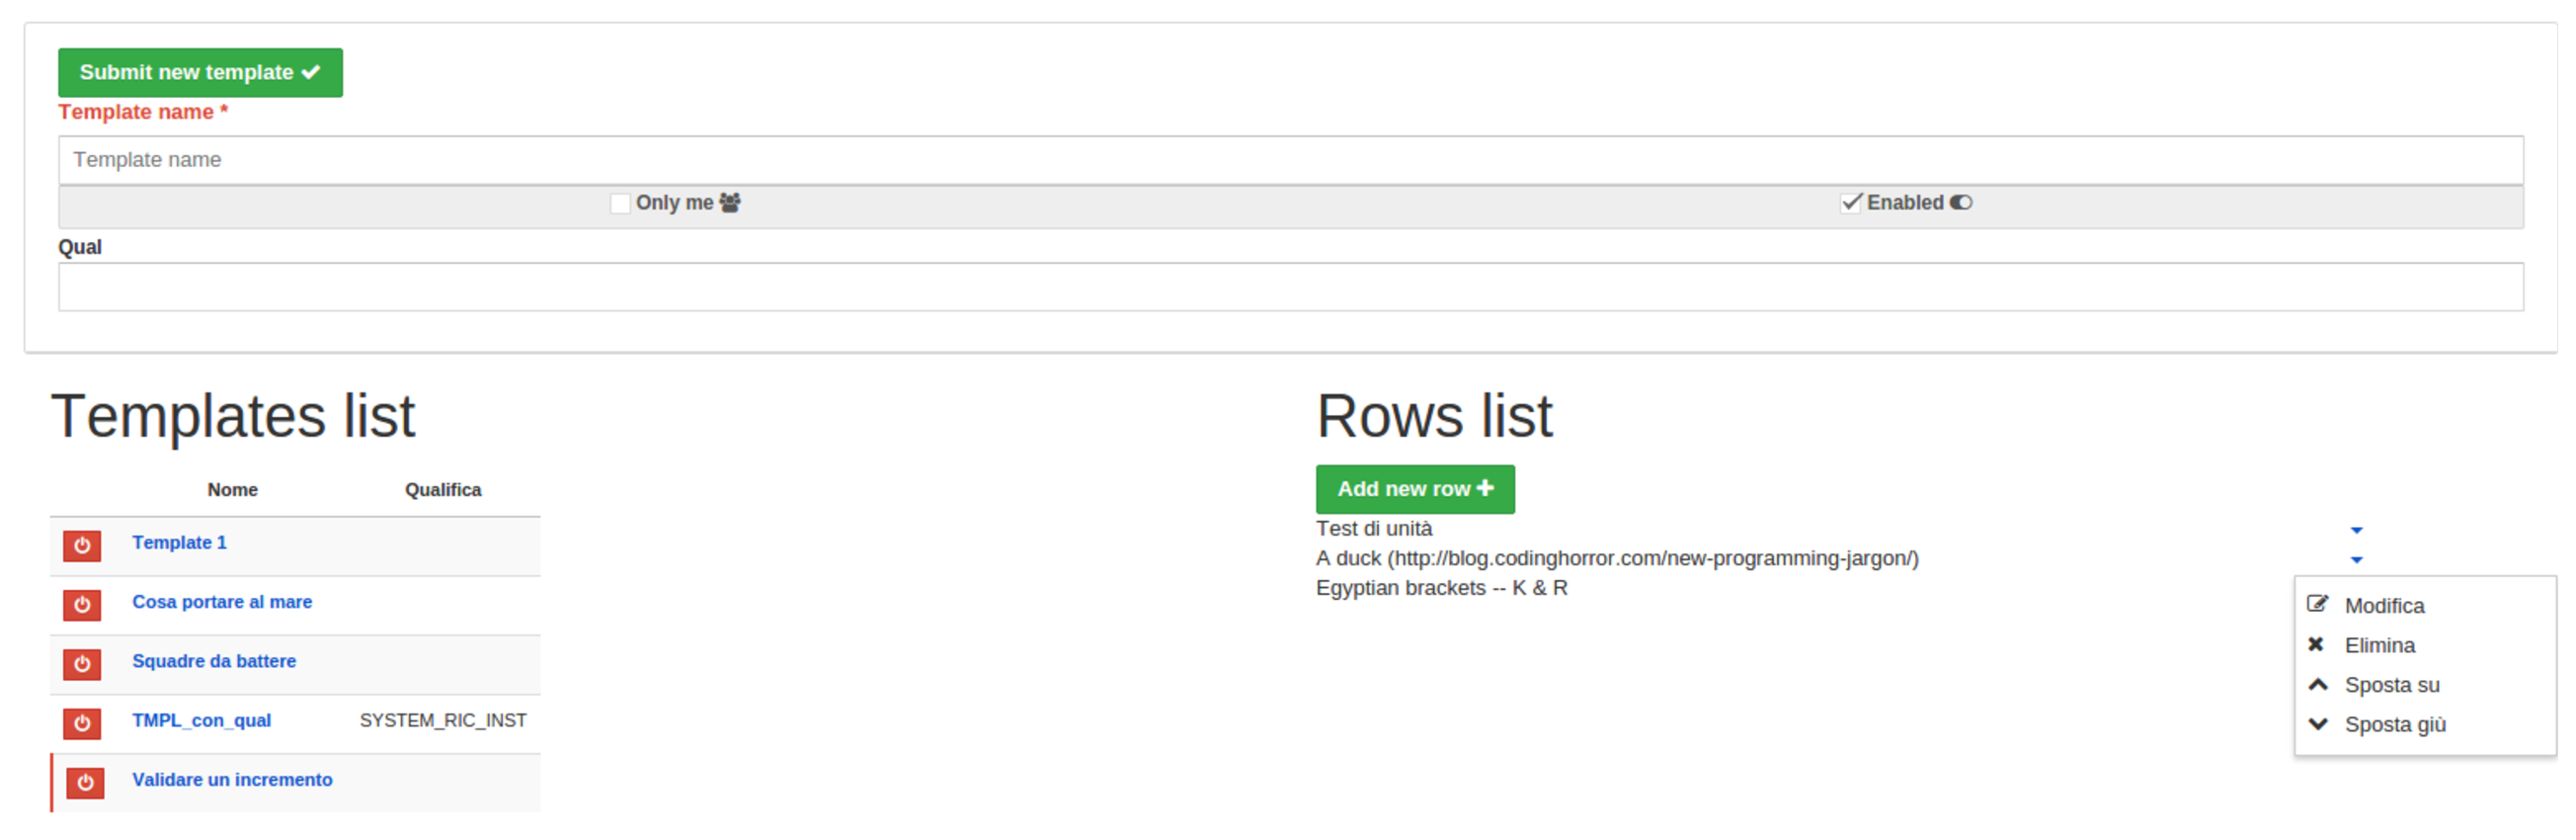
\includegraphics[width=1.2\columnwidth]{immagini/clTemplate}
    \caption{Modulo di gestione template di checklist}
    \label{fig:gestione-tmpl-cl}%
    \end{figure}
  % FINE GESTIONE TEMPLATE CL
  % DIRETTIVA CHECKLIST
  \item \Gloss{direttiva} riusabile in altre parti di JPA (fig.
    \ref{fig:cl-in-viewer}).
    \begin{figure}[H]%
    \centering
    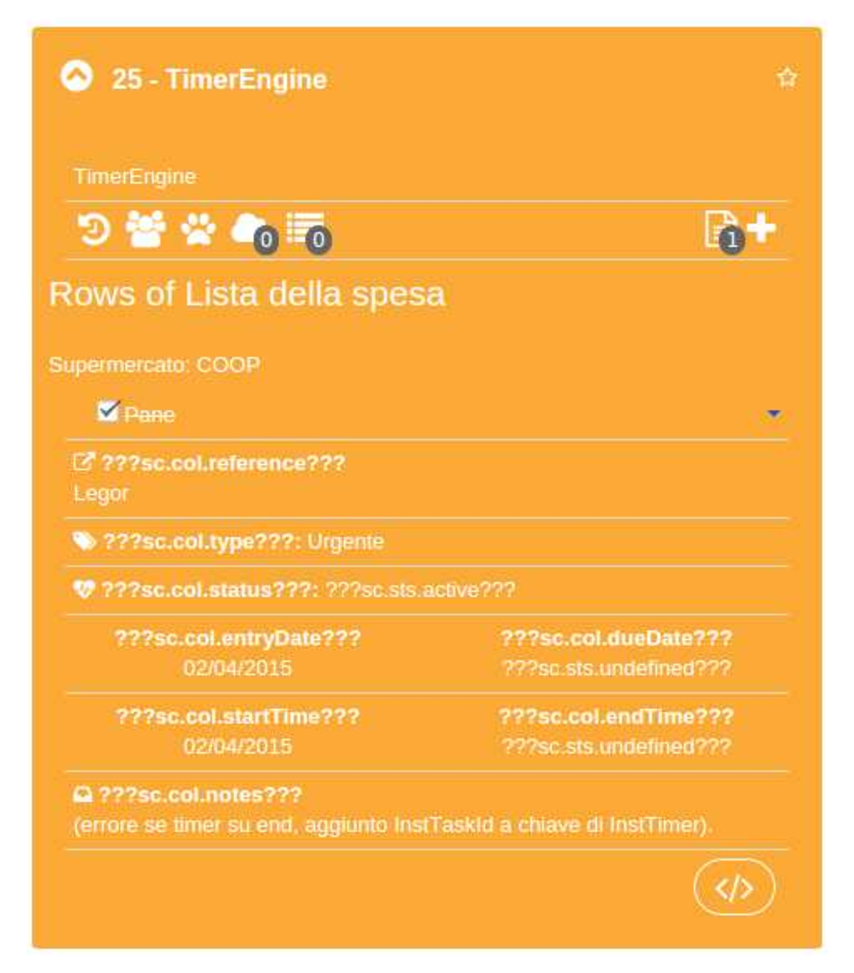
\includegraphics[width=.5\columnwidth]{immagini/taskConChecklist}
    \caption{\Gloss{direttiva} per le checklist usata in un task}
    \label{fig:cl-in-viewer}%
    \end{figure}
  % FINE DIRETTIVA CHECKLIST
  \end{itemize}
\item \textbf{Burn-down chart:}
  \begin{itemize}
  \item \Gloss{direttiva} riusabile in altre parti di JPA (fig.
    \ref{fig:bdchart});
  \end{itemize}
\item \textbf{Strumenti di \emph{Inspection}:}
  \begin{itemize}
  \item Modulo contenente burn-up chart (fig. \ref{fig:burnup}), cumulative
    flow diagram (fig. \ref{fig:cumulative}) e pie chart sulla ripartizione
    dei task (fig. \ref{fig:pies}).
    % PIES
    \begin{figure}[H]
      \subfloat[Grafico a torta per livelli\label{fig:pies-types}]{%
        \includegraphics[width=.5\textwidth]{immagini/LevelsPieCurrent}
      }
      \vspace*{\fill}
      \subfloat[Grafico a torta per tipi\label{fig:pies-lev}]{%
        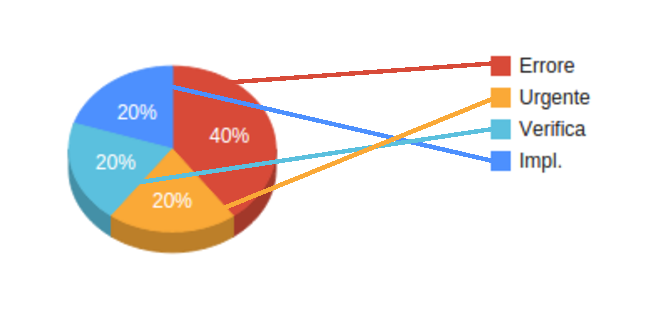
\includegraphics[width=.5\textwidth]{immagini/TypesPieStart}
      }
      \caption{Pie chart}
      \label{fig:pies}
    \end{figure}
    % FINE PIES
  \end{itemize}
\item \textbf{Avvio istanza di processo:}
  \begin{itemize}
  % AVVIO ISTANZA
  \item Modifiche a moduli del \FREND{}.
    \begin{figure}[H]%
    \centering
    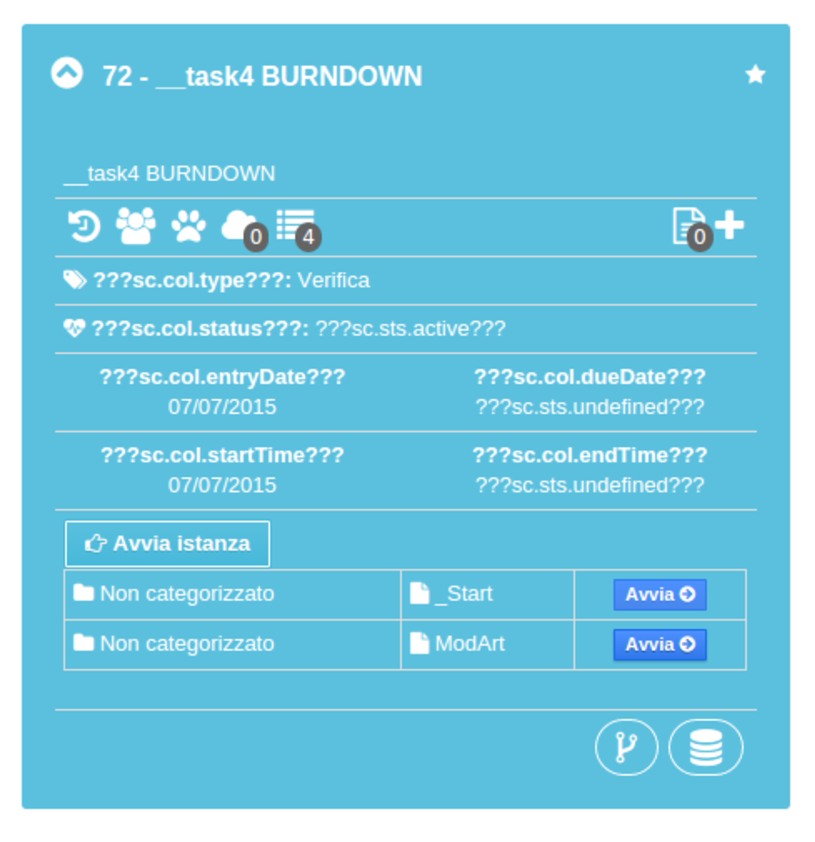
\includegraphics[width=.8\columnwidth]{immagini/avvioIstanza}
    \caption{Avvio istanza da task}
    \label{fig:avvio-istanza-task}%
    \end{figure}
  % FINE AVVIO ISTANZA
  \end{itemize}
\item \textbf{Realizzazione di \gloss{api} per l'area Scrum:}
  \begin{itemize}
  \item Modifiche a una classe di utilità nel \BKEND{}.
  \end{itemize}
\item \textbf{Funzionalità di notifica:}
  \begin{itemize}
  % CONFIGURAZIONE NOTIFICHE
  \item Sezione dedicata a configurazione notifiche (fig.
    \ref{fig:config-testo-notifiche});
    \begin{figure}[H]%
    \centering
    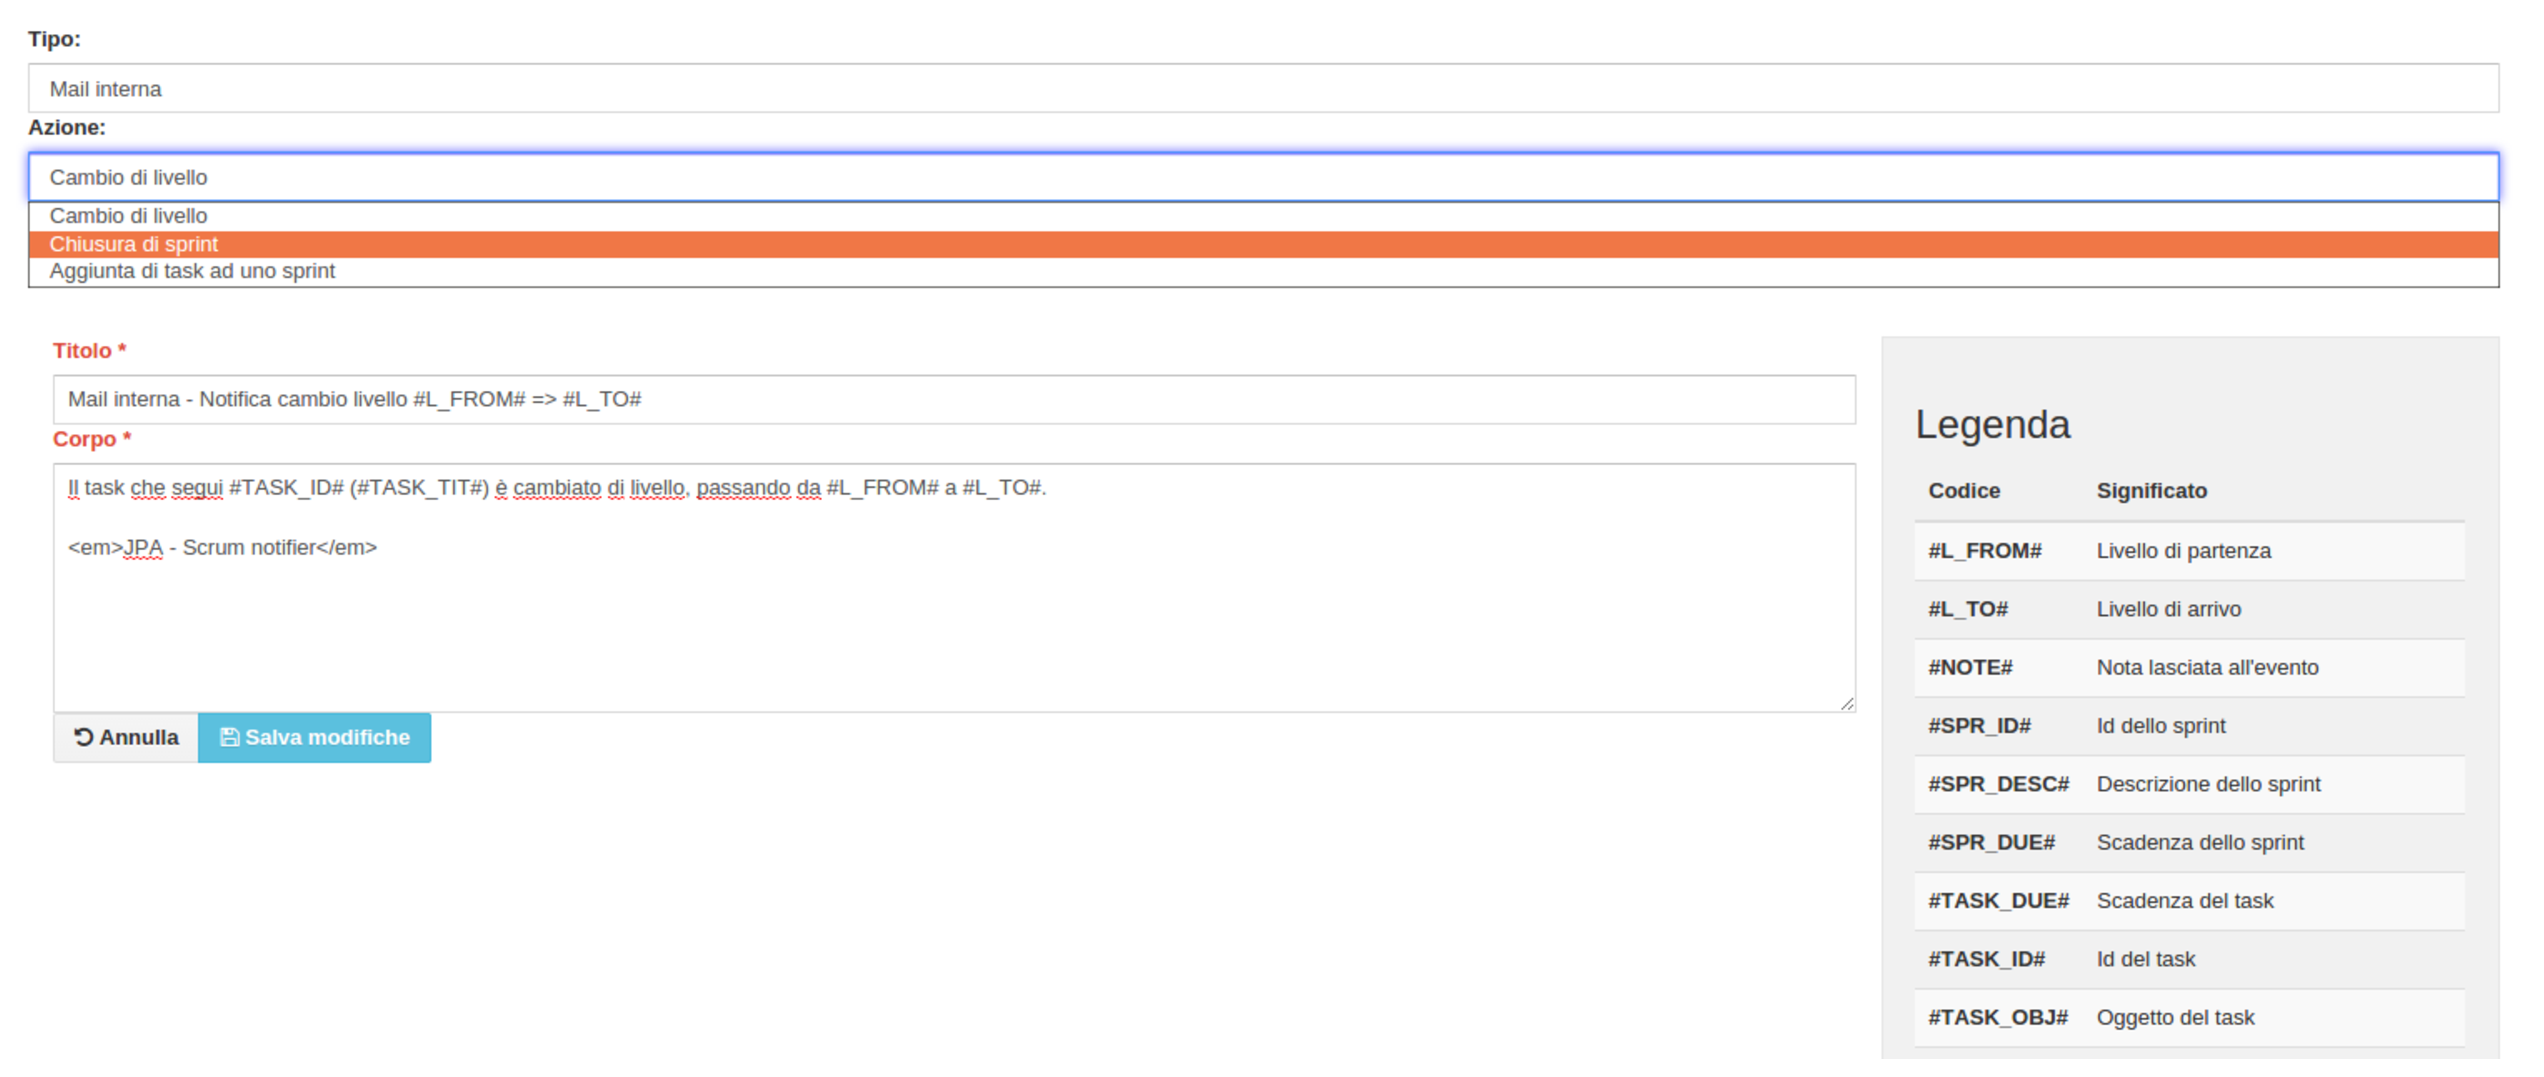
\includegraphics[width=1.2\columnwidth]{immagini/configurazioneNotifiche}
    \caption{Configurazione testo notifiche}
    \label{fig:config-testo-notifiche}%
    \end{figure}
  % FINE CONFIGURAZIONE NOTIFICHE
  % ATTIVAZIONE NOTIFICHE
  \item Attivazione notifiche in moduli (fig. \ref{fig:attivazione-notifiche});
    \begin{figure}[H]%
    \centering
    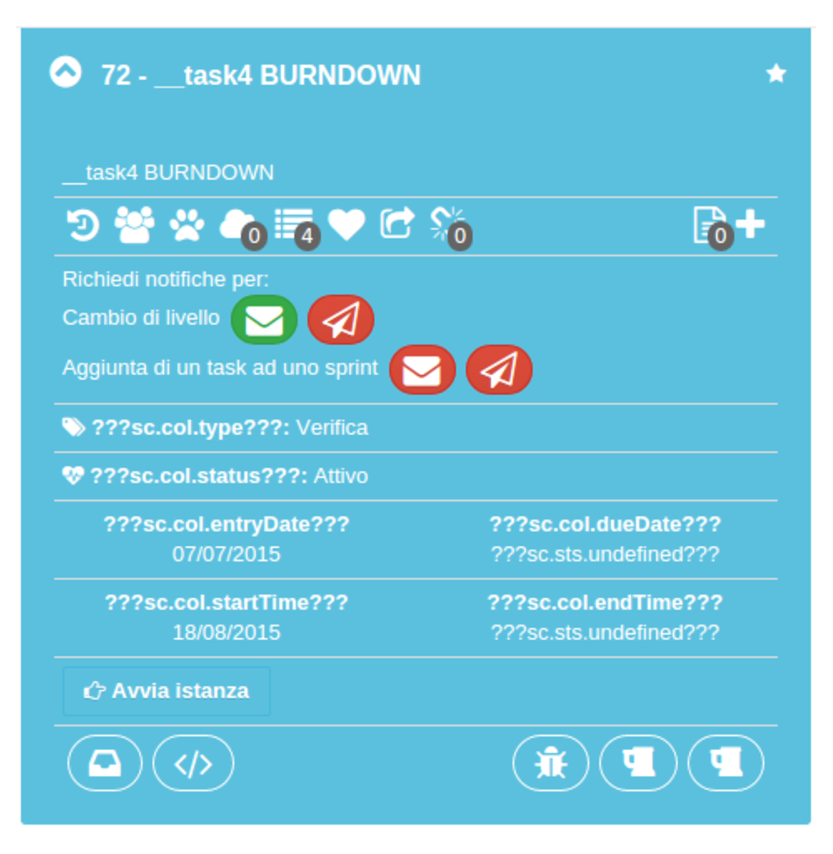
\includegraphics[width=.8\columnwidth]{immagini/attivazioneNotifiche}
    \caption{Attivazione notifiche nel visualizzatore di sprint}
    \label{fig:attivazione-notifiche}%
    \end{figure}
  % FINE ATTIVAZIONE NOTIFICHE
  \item Ricezione notifica via mail interna e via Telegram (fig.
    \ref{fig:screen-telegram}).
  \end{itemize}
\item \textbf{Collegamento al forum:}
  \begin{itemize}
  % DISCUSSIONE FORUM
  \item Modifiche ai moduli per permettere l'apertura di discussioni in forum.
    \begin{figure}[H]%
    \centering
    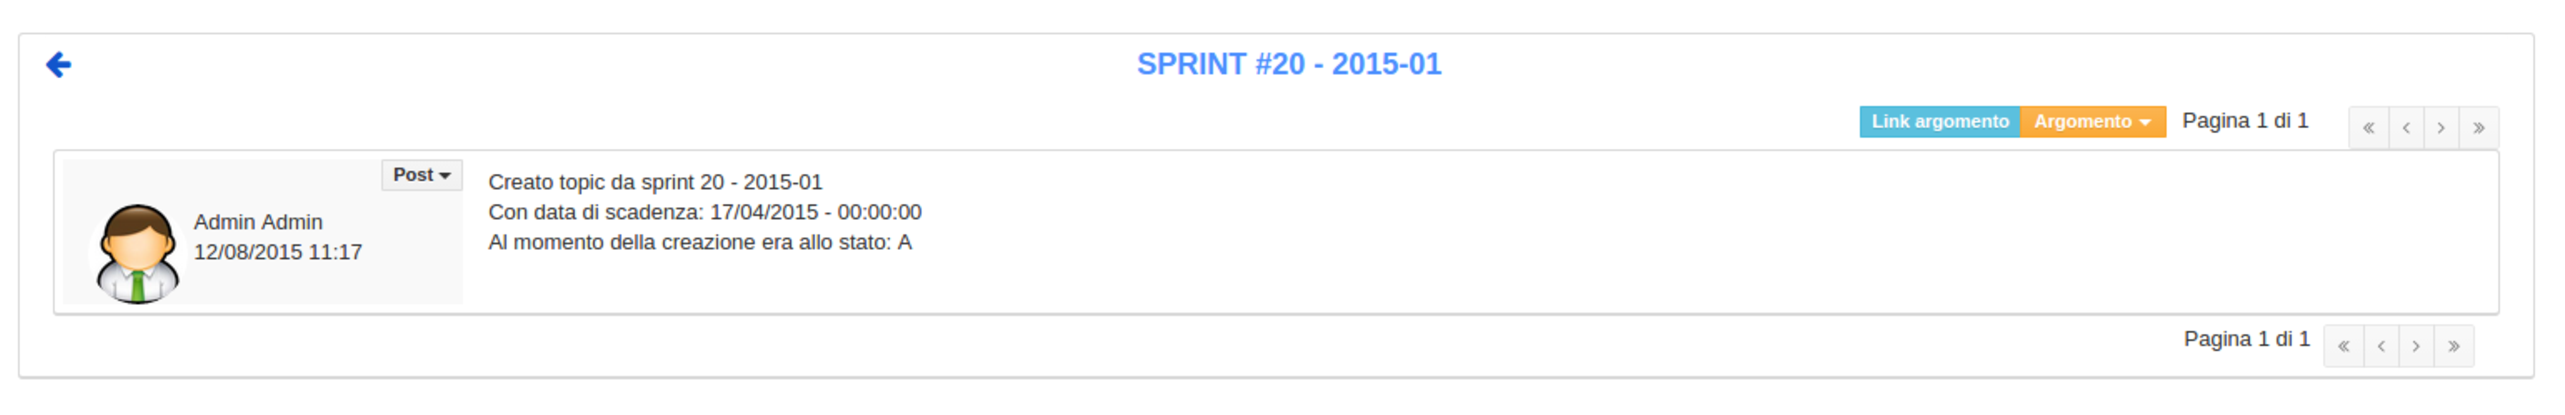
\includegraphics[width=1.2\columnwidth]{immagini/discussioneInForum}
    \caption{Discussione in area Forum aperta da sprint}
    \label{fig:discussione-forum}%
    \end{figure}
  % FINE DISCUSSIONE FORUM
  \end{itemize}
\item \textbf{Sviluppi ulteriori:}
  \begin{itemize}
  \item Incrementi relativi ai Telegram Bot.
  \end{itemize}
\end{itemize}
